\documentclass{article}

% ================================================================
% ICLR 2027 draft (2026-07-25), converted from softprompting_icml.tex.
% Changes vs. the ICML version:
%   * ICLR (single-column) format; iclr2027_conference.sty is the official
%     ICLR 2026 style with the year string patched (2027 files not yet
%     released; swap in the official ones when available).
%   * Matched-input headline: Figure 1 and Table 1 show the LoRA
%     class-names sweep only and the fixed-IST SoftPrompt only.
%     Instruction-augmented LoRA (unmatched input) and best-of-IST/TSI
%     live in the appendix, with a fairness note in Sec. 4.2.
%   * Figure 1 regenerated by
%     code/generate_accuracy_forgetting_figure.py --fair
%     -> paper/figures/AccuracyForgettingVsParams_fair.{png,pdf}
% Compile from the repo root:
%   pdflatex paper/softprompting_iclr.tex
% ================================================================

\usepackage{paper/iclr2027_conference,times}
% \iclrfinalcopy % Enable only for the camera-ready version.

\usepackage{microtype}
\usepackage{graphicx}
\usepackage{subcaption}
\usepackage{booktabs}
\usepackage{multirow}
\usepackage{makecell}
\usepackage{hyperref}
\usepackage{url}
\usepackage{amsmath}
\usepackage{amssymb}
\usepackage{amsfonts}
\usepackage{nicefrac}
\usepackage{xcolor}
\usepackage{tikz}
\usetikzlibrary{positioning}
\usetikzlibrary{decorations.pathreplacing}
\usetikzlibrary{arrows.meta}
\usepackage{pgfplots}
\pgfplotsset{compat=1.18}

% Convenience macros
\newcommand{\ours}{\textsc{SoftPrompt}}
\newcommand{\lora}{\textsc{LoRA}}
\newcommand{\distill}{\textsc{Soft2Hard}}
\newcommand{\zeroshot}{\textsc{Zero-shot}}
\newcommand{\hard}{\textsc{HardPrompt}}
\newcommand{\qwen}{Qwen3-VL}
\newcommand{\rftwenty}{Roboflow20-VL}
\newcommand{\eg}{\textit{e.g.}}
\newcommand{\ie}{\textit{i.e.}}
\definecolor{ours_color}{RGB}{22, 96, 165}
\newcommand{\best}[1]{\textbf{#1}}
\newcommand{\second}[1]{\underline{#1}}

% Author notes (strip before submission)
\newcommand\grg[1]{\textcolor{purple}{[GRG: #1]}}
\newcommand\deva[1]{\textcolor{blue}{[Deva: #1]}}
\newcommand\john[1]{\textcolor{red}{[John: #1]}}


% Finding box: one boxed claim (with its number) per result-bearing section.
% Per-section key-finding callout, package-free.
\definecolor{findingframe}{RGB}{38,148,132}
\definecolor{findingback}{RGB}{233,247,244}
\newsavebox{\findingbox}
\newenvironment{finding}
  {\par\smallskip\noindent\begin{lrbox}{\findingbox}%
   \begin{minipage}{\dimexpr\linewidth-2\fboxsep-2\fboxrule\relax}\small}
  {\end{minipage}\end{lrbox}%
   \setlength{\fboxrule}{0.9pt}%
   \noindent\fcolorbox{findingframe}{findingback}{\usebox{\findingbox}}\par\smallskip}

\title{ \begin{center} {\LARGE \begin{tabular}{@{}c c c@{}} \multirow{2}{*}{\includegraphics[height=2.1em]{paper/figures/TitleEmoji_teach.png}} & Your Model Already Knows & \multirow{2}{*}{\includegraphics[height=2.1em]{paper/figures/TitleEmoji_ask.png}} \\ & Don't Teach It, Learn to Ask It & \end{tabular} }\par\vspace{0.1em} {\large Soft Prompting for Few-Shot Adaptation of\\[-0.1em] Vision-Language Models} \end{center} }

\author{Anonymous authors\\
Paper under double-blind review}

\begin{document}

\maketitle

\begin{abstract}
Few-shot adaptation of vision-language models (VLMs) is difficult for
specialized aerial, industrial, medical, and other imagery when only ten
annotated images are available.
Discrete prompt optimizers such as GEPA, DetPO, and TextGrad keep the model
frozen and produce readable text, but do not optimize continuous embeddings by
numerical gradient descent; low-rank adapters use gradient descent effectively
but learn millions of task-specific parameters.
We revisit soft prompting, which combines these benefits by optimizing a small
continuous input while keeping the pretrained backbone frozen.
We find that two design choices unlock its performance: initializing from a
semantically empty space token and placing learned tokens at the cross-modal
boundary in the gradient path of the target output.
The latter principle is not specific to detection.
We evaluate on \rftwenty{}, where the resulting prompt uses $7{,}168$ trainable
parameters on average, outperforms GEPA and DetPO under the shared multi-class
protocol, and matches the best class-name \lora{} configuration at $14.2$
mAP@50:95 with roughly $24{,}000\times$ fewer trainable parameters.
\distill{} further verbalizes the continuous prompt into an editable
instruction for human inspection.
On RoboCasa, a prompt that reaches the action expert raises two near-floor
tasks from $5.0\%$ success to $23.3\%$ and $31.7\%$, matching or exceeding
coverage-matched \lora{} with roughly $400\times$ fewer trainable parameters.
These results suggest that, when a VLM already contains the required knowledge,
few-shot adaptation can be a problem of learning how to ask.
\end{abstract}

\section{Introduction}
\label{sec:intro}

Vision-language models (VLMs) trained on web-scale data recognize common
objects, yet often fail on specialized imagery such as aerial surveys,
industrial inspection, and medical scans
\citep{Radford2021LearningSupervision,Bai2023Qwen-VL:Beyond,Robicheaux2025Roboflow100-VL:Models}.
When only ten labeled images are available, the central question is how much
task-specific machinery should be learned.

Existing approaches occupy two ends of a spectrum.
Discrete prompt optimization, including GEPA
\citep{AgrawalGEPA:LEARNING}, DetPO
\citep{Gare2026DetPO:Detection}, and TextGrad
\citep{yuksekgonul2024textgrad}, keeps the VLM frozen and searches over
human-readable tokens, but does not apply numerical gradient descent to
continuous prompt embeddings.
\lora{} \citep{Hu2021LoRA:Models} instead freezes the pretrained matrices and
learns low-rank factors whose updates are active with the adapter; it supports
gradient descent but introduces a task-specific parameter block at many
transformer layers.
Soft prompting combines the relevant benefits: like \lora{}, it optimizes
continuous parameters by numerical gradient descent; like prompting, it leaves
the pretrained backbone frozen and attaches task-specific state only at the
input.

\begin{figure}[t]
  \centering
  \includegraphics[width=0.76\textwidth]{paper/figures/AccuracyForgettingVsParams_fair.pdf}
  \caption{\textbf{\ours{} reaches the class-name \lora{} accuracy frontier
  with far fewer trainable parameters; active \lora{} adapters exhibit
  rank-dependent cross-task interference.}
  \emph{Top:} RF20 10-shot mAP@50:95 under the shared class-name protocol.
  \emph{Bottom:} mean relative NaturalBench G-Acc change over 20 independently
  trained RF20 \lora{} adapters left active at each rank. Disabling \lora{}
  restores the base computation, just as omitting a soft prompt does; no
  matched active-conditioning SoftPrompt point is claimed.}
  \label{fig:pareto}
\end{figure}

Soft prompting is not automatically effective in a multimodal autoregressive
sequence.
Common prompt- and prefix-tuning formulations inherited from NLP place learned
vectors before the textual context
\citep{LesterTheTuning,li2021prefix}, even though a VLM contains distinct
visual and textual spans and therefore several possible boundaries.
We find that placing the tokens at the cross-modal boundary and initializing
them to preserve the original prompt semantics are the enabling choices.
With these choices, \ours{} uses one to three learned tokens per domain and
reaches $14.2$ mAP on \rftwenty{}, matching the best class-name configuration
in a six-rank \lora{} sweep and exceeding multi-class DetPO by $1.7$ mAP
(Figure~\ref{fig:pareto}).

Continuous tokens are compact but normally opaque.
Our \distill{} procedure asks the VLM to verbalize the task information elicited
by its learned prompt and produces an editable natural-language instruction
competitive with dedicated prompt search.
This does not prove that the text is a faithful causal explanation of each
embedding dimension, but it creates an artifact that can be inspected, revised,
documented, and reviewed in governed AI deployments.
The prompt-interpretation analysis in Appendix~\ref{app:analysis} further
studies cross-model transfer, and the robotics study in
Appendix~\ref{app:robotics} tests the placement principle on a robot policy.

\textbf{Contributions.}
(1) We present a soft-prompt method and practical few-shot training recipe
combining cross-modal placement, meaning-preserving initialization, short
length sweeps, and task-metric selection.
(2) In a controlled RF20 comparison with prompt search, six \lora{} ranks, and
a specialist detector, \ours{} matches the best class-name \lora{} result with
roughly $24{,}000\times$ fewer trainable parameters.
(3) We introduce \distill{}, which produces an editable text artifact, and use
RoboCasa to test whether the gradient-path placement principle transfers
beyond detection.

\section{Related Work}
\label{sec:related}

\textbf{VLM detection.}
Generative VLMs such as \qwen{} \citep{Bai2023Qwen-VL:Beyond}, LLaVA
\citep{Liu2023VisualTuning}, and InstructBLIP \citep{instructblip} emit
detections as structured text.
Specialist open-vocabulary detectors such as Grounding DINO
\citep{Liu2023GroundingDetection} and OWL-ViT \citep{owlvit} align regions with
text and remain stronger in raw detection accuracy; we include them to delimit
our claim about adapting a general-purpose VLM.

\textbf{Prompt tuning and PEFT.}
Prompt tuning \citep{LesterTheTuning}, prefix tuning \citep{li2021prefix},
VPT \citep{jia2022vpt}, and CoOp/CoCoOp
\citep{ZhouLearningModels,cocoop} learn continuous prompts for frozen models.
Unlike deep variants that inject parameters at every layer, our shallow prompt
enters once, and its position relative to visual and text tokens is a
first-class design variable.
\lora{} \citep{Hu2021LoRA:Models} and adapters \citep{adapters} are
parameter-space alternatives that learn task-specific modules while retaining
the pretrained matrices.

\textbf{Discrete prompt optimization.}
GEPA \citep{AgrawalGEPA:LEARNING} evolves prompts, TextGrad
\citep{yuksekgonul2024textgrad} propagates language critiques, AutoPrompt
\citep{Shin2020AutoPrompt:Prompts} performs gradient-guided token search, and
DetPO \citep{Gare2026DetPO:Detection} specializes discrete search to detection.
These methods preserve readable tokens but search a discrete space; our method
uses gradients in continuous embedding space and then recovers an editable
hard prompt through \distill{}.
Additional work on distillation and transfer appears in
Appendix~\ref{app:analysis}.

\section{Method}
\label{sec:method}

\subsection{Soft tokens at the cross-modal boundary}
\label{subsec:method_position}

A VLM $f_\theta$ encodes an image as $N_I$ patch embeddings
$\mathbf{I}\in\mathbb{R}^{N_I\times d}$ and a query as $N_T$ token embeddings
$\mathbf{T}\in\mathbb{R}^{N_T\times d}$, then emits detections as structured
text.
We add $L$ trainable embeddings
$\mathbf{S}\in\mathbb{R}^{L\times d}$.
Image (I), soft (S), and text (T) spans admit six orderings: IST, TSI, ITS,
TIS, SIT, and STI.
Our default places the prompt between modalities,
\begin{equation}
  \widetilde{\mathbf{X}}=[\mathbf{I};\mathbf{S};\mathbf{T}],
  \label{eq:ist}
\end{equation}
so the learned tokens follow every visual patch and precede every query token.
The six orderings separate three qualitatively different interventions.
SIT and STI transpose the standard NLP prefix into a multimodal sequence,
placing the learned state before either observed modality. ITS and TIS make it
a suffix, after both modalities have already entered the causal stream. IST
and TSI instead place the trainable block at a modality boundary. In IST, the
prompt can be conditioned by all preceding visual patches while affecting
every following query token. This makes the block a plausible bottleneck for
domain-specific visual evidence, rather than an unconditional prefix.

This argument motivates rather than proves the choice. Attention can carry
information across positions, and the preferred ordering may depend on the
backbone's serialization and attention masks. We therefore treat ordering as
an empirical design variable, evaluate all six possibilities, and use IST as
the fixed default only after the controlled comparison.
This cross-modal rationale motivates IST; Section~\ref{subsec:position}
evaluates rather than assumes its advantage.
Figure~\ref{fig:overview} summarizes the resulting input sequence and training
boundary; Appendices~\ref{app:gradflow} and~\ref{app:vllm} detail gradient flow
and serving with a standard inference engine.

\begin{figure}[t]
  \centering
  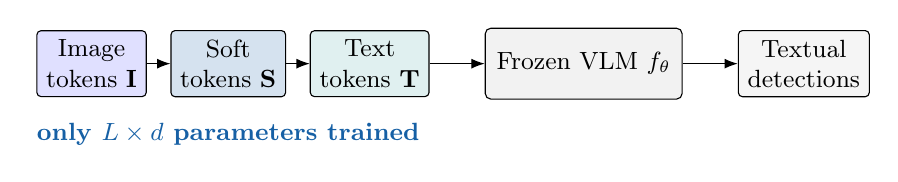
\begin{tikzpicture}[
    node distance=3mm,
    token/.style={draw, rounded corners=1.5pt, minimum height=7mm,
                  minimum width=13mm, align=center, font=\small},
    model/.style={draw, rounded corners=2pt, fill=gray!10,
                  minimum height=9mm, minimum width=25mm, font=\small},
    >=Latex]
    \node[token, fill=blue!12] (image) {Image\\tokens $\mathbf I$};
    \node[token, fill=ours_color!18, right=of image] (soft)
      {Soft\\tokens $\mathbf S$};
    \node[token, fill=teal!12, right=of soft] (text)
      {Text\\tokens $\mathbf T$};
    \node[model, right=7mm of text] (vlm) {Frozen VLM $f_\theta$};
    \node[token, fill=gray!8, right=7mm of vlm] (out) {Textual\\detections};
    \draw[->] (image) -- (soft);
    \draw[->] (soft) -- (text);
    \draw[->] (text) -- (vlm);
    \draw[->] (vlm) -- (out);
    \node[ours_color, font=\small\bfseries, below=2mm of soft]
      {only $L\times d$ parameters trained};
  \end{tikzpicture}
  \caption{\textbf{\ours{} inserts a small learned block at the cross-modal
  boundary.} The pretrained VLM remains frozen; gradients update only
  $\mathbf S$.}
  \label{fig:overview}
\end{figure}

\subsection{Optimization and initialization}
\label{subsec:method_training}
\label{subsec:method_init}

Given the 10-shot support set $\mathcal D$, training uses the backbone's
next-token detection loss while freezing $\theta$:
\begin{equation}
  \min_{\mathbf S}\mathcal L_{\mathrm{det}}(\mathbf S;\mathcal D,f_\theta).
  \label{eq:loss}
\end{equation}
More explicitly, for an image--query pair with target detection string
$\mathbf y=(y_1,\ldots,y_M)$, we minimize
\begin{equation}
  \mathcal L_{\mathrm{det}}(\mathbf S;\theta)
  =-\sum_{m=1}^{M}\log p_\theta
    (y_m\mid y_{<m},\mathbf I,\mathbf S,\mathbf T),
  \qquad \theta\ \text{fixed}.
  \label{eq:autoregressive_loss}
\end{equation}
The backbone parameters remain constants in this objective. The prompt
gradient,
$\nabla_{\mathbf S}\mathcal L_{\mathrm{det}}$, nevertheless includes the
Jacobian of every frozen transformer block between the input and the emitted
detection tokens. ``Frozen'' therefore means that those blocks retain no
updates, not that they disappear from forward or backward computation.
The target is the same structured sequence used by the frozen detector:
class labels and normalized bounding-box coordinates are generated
autoregressively. No detection head, visual projection, or pretrained
embedding row is updated. Gradients still traverse the complete VLM, but only
the new rows in $\mathbf S$ retain updates.

This gives SoftPrompt and \lora{} different optimization geometry.
\lora{} installs trainable low-rank factors at attention and MLP projections
throughout the decoder, so trainable parameters receive local gradient signals
at many depths. SoftPrompt has one input-side trainable sink at the far end of
the backward path. Its parameter footprint is much smaller, but its influence
must propagate through every frozen layer. This distinction motivates both
careful placement and a conservative initialization; it also explains why few
trainable parameters do not imply proportionally lower activation memory.
Appendix~\ref{app:gradflow} visualizes the two gradient paths.

For \qwen{}-8B, $d=4096$: $L=1$, $L=2$, and $L=3$ contain $4{,}096$,
$8{,}192$, and $12{,}288$ trainable parameters, respectively.
The selected per-domain lengths average $L=1.75$, or $7{,}168$ parameters.
We initialize every row of $\mathbf S$ with the embedding of a space token.
Unlike class names or task descriptions, this start is intended to leave the
original query semantics nearly unchanged and let optimization introduce only
the task-specific signal supported by the ten examples.
The design follows the residual-learning principle of beginning near an
already useful computation. A semantic seed such as a class name or the word
\texttt{detect} changes the query before seeing any evidence that the change is
helpful; optimization must then preserve useful meaning, erase harmful
meaning, and fit the task simultaneously. A whitespace embedding instead
starts close to the original class-name query and asks the optimizer to learn
only the residual task information.
We test this claim against Xavier-uniform, mean-vocabulary, class-seeded, and
task-text initializations. Copying the space embedding does not make the
initial prompt exactly invisible to every layer because it still occupies
positions in the sequence, but it avoids asserting a new lexical instruction before
training begins. We therefore call it meaning-preserving rather than
function-preserving.

\subsection{From continuous to editable prompts}
\label{subsec:method_distill}

\distill{} exposes the learned prompt through the model's own language.
Directly asking what an isolated embedding means is ill-posed: the prompt was
optimized only in the joint context of an image and detection query, and its
nearest vocabulary token need not express its contextual effect. We therefore
read out behavior rather than assign a word to each vector.

The procedure has three stages. First, with the learned prompt active, the VLM
describes the target objects in every support image before producing
detections. Second, a text-only pass summarizes these descriptions into one
global detection instruction. Third, that instruction replaces the soft
tokens and is evaluated with the unmodified base VLM. The deployed artifact is
therefore ordinary text: it can be inspected, edited, versioned, or passed to a
model API that exposes no embedding interface.

The same generate--summarize--evaluate pipeline is run without soft tokens.
This control matters because descriptions of labeled support images can improve
a prompt even when no learned embedding contributes information. The
soft-source minus base-source difference isolates what the continuous prompt
adds to the otherwise identical verbalization recipe. This is a behavioral
readout, not a claim that the resulting sentence is a faithful causal
decomposition of the embedding coordinates.
Both source conditions use the same support images, generation request,
summarizer, and downstream detection template. Only the presence of
$\mathbf S$ during description generation changes. At evaluation, neither
condition contains soft tokens, so any difference must pass through the
natural-language artifact. This makes the control stricter than comparing the
distilled prompt only with the original class-name query.
Appendix~\ref{app:analysis} gives the full procedure and analyses.

\section{Experiments}
\label{sec:experiments}

\subsection{Setup}
\label{subsec:setup}

\textbf{Benchmark and models.}
\rftwenty{} is a 20-domain subset of Roboflow-100-VL
\citep{Robicheaux2025Roboflow100-VL:Models} spanning aerial, document, flora
and fauna, industrial, medical, sports, and other imagery.
Each domain supplies ten support images and a held-out test split.
Main results use \qwen{}-8B-Instruct and COCO mAP@50:95 on a 0--100 scale.
The VLM receives one image and a class-name query, then emits all detections in
one structured response. We parse class labels and normalized coordinates and
score them with the same evaluator for every generalist method. Category
columns average datasets within each of the benchmark's seven
super-categories; ``All'' gives equal weight to each of the 20 domains.
Appendix~\ref{app:lvis} reports a higher-baseline LVIS Rare 50 check, and
Appendix~\ref{app:gemma4} trains the recipe on the unrelated
Gemma-4-12B-it family.

\textbf{Baselines.}
\hard{} queries the frozen VLM with class names or hand-written instructions.
GEPA and DetPO optimize discrete prompts on the same frozen backbone.
For matched input, \lora{} uses the class-name protocol and sweeps ranks
$4,8,16,32,64,128$; it freezes pretrained matrices and trains low-rank factors
on attention and MLP projections.
Every rank uses the same 10-shot support images, optimizer budget, generation
template, and test evaluator. The rank sweep is important because selecting
only one conventional rank could make a parameter-efficiency comparison
arbitrary: here accuracy rises through $r=64$ and falls at $r=128$.
Grounding DINO is a specialist reference, not a parameter-matched generalist.
All main generalist rows use one multi-class query per image; DetPO's
published single-class protocol reaches $17.5$ mAP with VQA-score reranking,
but requires one call per class and is not inference-cost-comparable
(Appendix~\ref{app:single_class}).

\textbf{Comparison scope.}
The comparison separates three costs that are often conflated. ``Params''
counts task-specific values learned by gradient descent and stored after
training; it does not count the shared frozen backbone. Training-free prompt
optimizers consequently have zero trainable parameters, although their prompt
search still consumes model calls and their final text is processed at every
inference. SoftPrompt and \lora{} both store learned sidecars, but the former
stores only $L\times d$ input vectors while the latter stores low-rank factors
at many layers. Grounding DINO changes the model family and is included only to
show the accuracy available from a dedicated detector.

Input protocol is a second axis. The primary comparison uses class names and
one multi-class call for every generalist method. Hand-written instructions
change the available information, so instruction-augmented \lora{} is shown as
an unmatched reference rather than used to define class-name parity. Similarly,
DetPO's stronger single-class result is separated because its class-count
calls per image change inference cost. These distinctions prevent trainable
parameter count from standing in for all deployment cost.

\textbf{Training and selection.}
\ours{} uses AdamW, learning rate $5\times10^{-3}$, cosine scheduling, and
batch size 4.
Thirteen domains use a five-epoch budget; seven use a 50-epoch budget with
early stopping.
Together with space initialization, cross-modal placement, and a short length
sweep including $L=0$, these settings form our empirical recipe for observed
few-shot convergence problems, not a convergence guarantee.
\lora{} uses adapters on the decoder's attention and MLP projections, learning
rate $5\times10^{-5}$, cosine scheduling, 0.2 warmup, effective batch size 2,
and 70 optimizer steps. Both approaches use bf16 and seed 42 in the headline
comparison.
Appendix~\ref{app:best_config} gives the per-domain settings.
The main \ours{} row fixes IST and chooses $L$ per domain by test mAP from the
reported short length sweep; the $14.2$ result therefore includes
test-informed length selection.
\textbf{Disclosures.}
(i) Results are single runs in a regime with an estimated $20$--$28\%$
seed-to-seed spread (direct three-seed mean CV: $28\%$,
Appendix~\ref{app:seed_variance}); differences below roughly one mAP point
should be treated cautiously.
(ii) A further test-selected choice between IST and TSI reaches $14.7$ but is
used only for appendix analysis, never the headline comparison.

\textbf{Ablation pool.}
Controlled ablations use nine fixed datasets covering every super-category:
aerial-airport; actions; all-elements; defect-detection; dentalai;
flir-camera-objects; lacrosse-object-detection, a multi-class sports dataset;
new-defects-in-wood; and wb-prova.
Dentalai is the floor control; the other eight are the \emph{above-floor}
datasets used in win counts.
The pool is fixed across position, initialization, and length studies rather
than chosen separately for each conclusion. We report dentalai even though its
near-zero scores make wins unstable, and include it in numeric averages while
excluding it from win counts. All full tables retain the frozen $L=0$
class-name baseline so a learned prompt can be identified as harmful rather
than merely worse than another learned configuration.

\subsection{Main RF20 results}
\label{subsec:main}

\begin{table}[t]
  \centering
  \caption{\textbf{\ours{} matches the best class-name \lora{} configuration
  on \rftwenty{} 10-shot.}
  Category-level mAP@50:95; All averages 20 datasets.
  \best{Bold}: best result within the matched class-name protocol; the
  instruction-augmented \lora{} row is an unmatched reference.}
  \label{tab:rf20_categories}
  \small
  \setlength{\tabcolsep}{3.5pt}
  \resizebox{\textwidth}{!}{%
  \begin{tabular}{lc|ccccccc|c}
    \toprule
    Method & Params & Aerial & Doc. & F.\,\&\,F. & Ind. & Med. & Sports & Other & All \\
    \midrule
    \hard{} (class names)                 & 0      &  6.4 &  7.5 & 25.0 & 8.2 & 0.0 &  8.6 &  9.1 & 10.8 \\
    \hard{} + instructions                & 0      &  7.4 &  8.5 & 25.0 & 9.1 & 0.2 &  9.7 &  9.6 & 11.3 \\
    GEPA \citep{AgrawalGEPA:LEARNING}     & 0      &  6.3 & 10.8 & 22.4 & 8.5 & 0.1 & 12.8 & 11.5 & 11.6 \\
    DetPO \citep{Gare2026DetPO:Detection} & 0      &  8.6 & 10.1 & 26.7 & \best{9.9} & 0.1 & 11.0 & 10.5 & 12.5 \\
    \midrule
    \ours{} (IST, per-domain $L$)         & 7.2K   &  9.0 & 14.6 & 27.7 & 8.7 & 0.0 & \best{13.8} & \best{14.3} & \best{14.2} \\
    \lora{} ($r=64$)                      & 174.6M & \best{20.2} & \best{19.9} & \best{28.6} & 7.1 & \best{0.7} & 9.6 & 9.4 & \best{14.2} \\
    \lora{} + instructions ($r=32$)            & 87.3M & 15.0 & 17.8 & 27.9 & 12.8 & 0.5 & 10.8 & 11.8 & 14.8 \\
    \midrule
    Grounding DINO (zero-shot)            & 0      & 31.2 & 5.0 & 34.3 & 13.0 & 0.4 & 5.7 & 16.9 & 17.3 \\
    Grounding DINO (10-shot fine-tune)    & 172M   & 40.6 & 32.0 & 44.9 & 41.0 & 35.3 & 30.8 & 26.8 & 35.7 \\
    \bottomrule
  \end{tabular}}
\end{table}

Table~\ref{tab:rf20_categories} shows the claimed middle ground in this
experiment: \ours{} uses numerical gradient descent and reaches the class-name
\lora{} frontier, but stores only 7.2K input parameters rather than a 174.6M
per-layer adapter.
\ours{} improves over training-free and discrete-search prompts by
$1.7$--$3.4$ mAP and equals the best class-name \lora{} rank at $14.2$
mAP@50:95 while training about $24{,}000\times$ fewer parameters.
Every other class-name rank is lower; the full \lora{} rank sweep is reported
in Appendix~\ref{app:lora_sweep}.
In a separate input protocol, the \lora{} model is trained and evaluated with
one multi-class query that appends each class's dataset description and
annotator instructions to the class names; its best rank reaches $14.8$
mAP@50:95. Because \ours{} was not trained with this enriched input, the row is
an unmatched reference rather than the basis of the $14.2$ parity claim.
This is parameter efficiency, not an assertion that \lora{} overwrites its
pretrained matrices: both methods learn removable task-specific state, but at
very different scales and locations.
The matched averages also conceal different category profiles. \lora{} is
substantially stronger on Aerial and Documents, while \ours{} leads on Sports
and Other. Their $14.2$ mAP@50:95 equality is therefore aggregate parity rather than
per-domain equivalence. The full rank sweep shows the same point from another
angle: adding adapter capacity is not monotonic, and the rank-128 model drops
to $13.6$ despite doubling the trainable parameters of rank 64.

The prompt baselines establish a second boundary. Hand-written class
instructions raise the frozen model from $10.8$ to $11.3$; GEPA reaches $11.6$
and multi-class DetPO $12.5$. In our experiments under the shared multi-class
protocol, numerical gradient descent on a continuous prompt closes a further
$1.7$ mAP gap from DetPO to the class-name \lora{} frontier.
DetPO's native single-class protocol reaches
$15.3$, or $17.5$ with reranking, showing that inference-time decomposition can
buy more accuracy when class-count scaling is acceptable. We do not use those
numbers to claim a same-cost win.

The storage consequence is concrete. The mean SoftPrompt checkpoint is
$29.6$KB, whereas the accuracy-matching rank-64 \lora{} adapter is $666.1$MB
(Appendix~\ref{app:vllm}). Both are removable sidecars, but the former makes
per-domain storage, routing, and copying inexpensive. This comparison concerns
task-specific state, not end-to-end training memory or latency.

The specialist detector defines the boundary.
Fine-tuned Grounding DINO reaches $35.7$ mAP, so practitioners seeking only
single-task detection accuracy should use a specialist.
The Medical category is sharper still: generalist prompts and adapters top out
at $1.0$ (Appendix~\ref{app:lora_sweep}), while the specialist reaches $35.3$.
Ten examples can steer knowledge already present in a general VLM, but cannot
reliably create missing domain knowledge.
Appendix~\ref{app:qual} shows the corresponding per-category qualitative
detections.

\subsection{Editable verbalization}
\label{subsec:distill}

Figure~\ref{fig:distill} shows the qualitative signal that \distill{} turns
into text.

\begin{figure}[t]
  \centering
  \includegraphics[width=0.92\textwidth]{paper/figures/DistillWithSoftTokens.png}
  \caption{\textbf{The learned prompt elicits a more specific description.}
  On the same aerial image, the prompt-active model identifies the object's
  relation to jet bridges; \distill{} summarizes descriptions like these into
  an editable detection instruction. This example illustrates inspectability,
  not a causal decoding of individual embedding dimensions.}
  \label{fig:distill}
\end{figure}

\distill{} reaches $12.5$ all-domain mAP as a plain-text prompt, matching DetPO
and exceeding GEPA, while remaining $2.2$ points below the $14.7$ test-selected
soft-prompt ceiling from which it is distilled.
The control is essential: the same describe-and-summarize pipeline without soft
tokens already reaches $12.2$, so the learned prompt adds only $+0.3$ on
average, concentrated in Aerial ($+4.1$) and Documents ($+2.6$).
This average is heterogeneous rather than a uniform small lift. The soft source
helps on 10 of 20 domains by $+1.9$ mAP on average and hurts on the remaining
10 by $-1.4$. The largest gains occur where the prompt-active descriptions add
concrete visual distinctions, such as the aircraft's relation to jet bridges
in Figure~\ref{fig:distill}. In domains the frozen model already
describes well, summarization can discard useful specificity.

The result is therefore not that every soft embedding has a literal textual
translation; rather, the learned prompt can contribute task information to a
human-readable artifact that remains useful without soft tokens.
Its $12.5$ mAP also identifies the cost of editability: it retains most, but
not all, of the $14.7$ source prompt's performance. That trade is useful when a
deployment values reviewability, provenance, or compatibility with text-only
interfaces more than the last points of task accuracy. Human readers can
inspect and revise the instruction, but should not interpret it as a complete
mechanistic explanation of the continuous prompt.
In particular, the distilled sentence explains a behavior observed under the
support-image context; it does not assign independent semantics to individual
prompt vectors. This distinction matters for audit use. A reviewer can inspect
whether the resulting instruction names inappropriate attributes, edit those
attributes, and rerun the downstream evaluation. They cannot infer from that
sentence alone why every detection changed. \distill{} therefore provides an
auditable interface and artifact, not a causal attribution method.
Full results and controls are in Appendix~\ref{app:analysis}; direct
soft-token transfer is compared with text-mediated transfer in
Appendix~\ref{app:distill_transfer}.

\subsection{Transfer across model versions}
\label{subsec:transfer_main}

A soft prompt is an input-side object rather than a set of changes tied to
particular transformer modules. This creates a simple, if demanding, transfer
test: load prompts trained on \qwen{}-8B directly into Qwen3.5-9B without a
learned projection or any target-model training. The dimensions are compatible,
but the embedding geometries need not be.

Across the 20 RF20 domains, direct transfer raises the 9B model from $9.9$ to
$10.7$ mAP. It helps 13 domains by $+2.9$ mAP on average and hurts seven by
$-3.1$, so the modest $+0.8$ aggregate is a mixture of meaningful gains and
losses rather than a uniformly small effect. The transferred prompt also
remains $4.0$ points below its $14.7$ source-model ceiling. Thus the embeddings
carry some model-independent domain signal, but much of their utility remains
coupled to the source model's geometry. Appendix~\ref{app:transfer} gives the
category breakdown, while Appendix~\ref{app:distill_transfer} compares direct
embedding transfer with using the distilled text as the transfer vehicle.
The category breakdown reinforces that conclusion: transfer helps most on
Sports ($+5.3$) and Documents ($+3.3$), but loses $2.9$ points on Industrial.
The sign is therefore domain-dependent even when source and target models come
from successive releases of the same family.

The target model's own unprompted score is the relevant denominator: the 9B
backbone does not preserve the 8B model's domain-by-domain strengths, so
comparing transferred scores only with the 8B origin would mix adaptation with
backbone differences. No projection, calibration set, or target-model gradient
step is used. The result is consequently a deliberately minimal transfer
baseline, not a claim that the two embedding spaces are aligned. Learning a
small cross-model projection is an obvious extension, but would introduce
target-model supervision absent from this test.

Transfer also exposes a tension between portability and fidelity. Text from
\distill{} is model-agnostic and can cross an API boundary, but compresses a
continuous representation into a short linguistic bottleneck. Raw embeddings
retain more of that representation, yet assume compatible hidden dimensions
and enough geometric alignment to remain meaningful. The appendix comparison
finds that direct embeddings usually outperform their own distilled
descriptions on the target model. Accordingly, text is the more portable
artifact, while vectors are the stronger transfer channel when compatible
models are available.

\section{Ablation Study}
\label{sec:ablations}

We isolate position, initialization, and length on the fixed nine-dataset pool.
All win counts exclude dentalai, the floor control, and all values are
mAP@50:95 from single runs.

\begin{table}[t]
  \centering
  \caption{\textbf{Cross-modal placement and meaning-preserving initialization
  unlock soft prompting.}
  Averages include all nine pool datasets; win counts exclude the dentalai
  floor control. Full per-dataset results and length curves are in
  Appendix~\ref{app:full_ablations}.}
  \label{tab:core_ablations}
  \small
  \setlength{\tabcolsep}{6pt}
  \begin{tabular}{llcc}
    \toprule
    Axis & Selected setting & Evidence & Practical conclusion \\
    \midrule
    Position & IST & 10.5 avg.; wins 5/8 & Test the cross-modal boundary \\
             & SIT (NLP prefix) & 9.6 avg.; wins 0/8 & Do not assume prefix placement \\
             & STI & 6.9 avg. (worst) & Best--worst spans ${\sim}6\times$ on lacrosse \\
    \midrule
    Initialization & Space token & 10.5 avg.; wins 5/8 & Start without adding semantics \\
                   & Xavier & 9.9 avg. & Semantic richness is not required \\
                   & Task text & 9.6 avg. & Task words can interfere initially \\
    \midrule
    Length & per-domain $L$ sweep & selected $L\in\{1,2,3\}$ & Include $L=0$ as a control \\
    \bottomrule
  \end{tabular}
\end{table}

\subsection{Injection position}
\label{subsec:position}

IST is best on five of eight above-floor datasets, improves over the frozen
baseline on seven, and is never the lowest-scoring ordering above the floor.
Neither soft-first prefix wins an above-floor dataset.
The strongest exception is informative: TSI wins aerial-airport, a
single-class task, while on the multi-class sports dataset lacrosse it falls
from IST's $24.0$ to $4.1$.
Thus IST is the robust default, with TSI worth testing when the text query
itself identifies the single target concept.

\subsection{Initialization and length}
\label{subsec:init}
\label{subsec:length}

The space token wins five of eight above-floor datasets and yields the best
average.
Semantic starts are less reliable: task-text initialization falls to $6.6$ on
lacrosse versus $24.1$ for space, while class-seeded initialization falls to
$5.3$ on all-elements versus $11.6$.
This supports a conservative start that preserves the existing query rather
than injecting an unvalidated semantic prior.

No universal length works.
Selected prompts use one to three tokens, but the sweep includes
$L\in\{0,1,2,3,4,8\}$ because a mis-sized prompt can underperform the frozen
$L=0$ control.
Length and position also interact: aerial degrades with longer IST prompts but
improves under TSI.
The practical recipe is therefore a short validation sweep that always
includes the unadapted model; our reported headline uses test-informed length
selection and should be read as an exploratory estimate.

\section{Discussion}
\label{sec:discussion}

\textbf{When does asking suffice?}
The aggregate result suggests that ten images often contain enough evidence to
steer knowledge already encoded by a general VLM.
The medical failure provides the counterexample: when the relevant visual
knowledge is absent, neither a tiny prompt nor a low-rank adapter recovers it,
and a specialist is appropriate.

This boundary suggests a staged adaptation strategy. Begin with a frozen-model
prompt because it is cheap to store, easy to remove, and sufficient when the
failure is one of elicitation. Escalate to a larger adapter when the prompt
plateaus despite stable validation evidence, and to a specialist when every
generalist method remains at the floor. The study does not establish that
parameter count alone selects among these regimes; it shows that a tiny
gradient-trained input should be included as a serious first-stage baseline.

The $14.2$ mAP@50:95 parity should likewise be interpreted at the level
supported by the experiment. It is parity between single-run aggregate scores, not evidence
that the two methods are interchangeable or statistically indistinguishable
on every domain. Their category profiles differ, and the three-seed study finds
substantially more variation for SoftPrompt. The result establishes that the
small prompt can reach the class-name \lora{} frontier under the explored
configuration space; repeated locked-test evaluation is needed to estimate the
expected gap.

\textbf{Practical recipe.}
Start with IST, space initialization, and
$L\in\{0,1,2,3,4,8\}$; select on held-out detection mAP rather than
language-model loss.
Treat TSI as a targeted alternative for single-class or text-dominant domains.
If a short sweep does not move the model off the floor, escalate to heavier
adaptation or a specialist rather than increasing prompt capacity blindly.
Keep the selected prompt, its textual distillation, the support examples, and
the evaluation report as separate versioned artifacts. The continuous prompt
preserves maximum accuracy, while the distilled instruction gives reviewers a
readable object that can be edited and re-evaluated. Neither should be treated
as self-certifying: the former is opaque, and the latter is only a behavioral
summary.

\textbf{Limitations.}
The main limitation is that soft prompts are harder to train than \lora{}:
SoftPrompt's seed-to-seed spread averages $7.9\times$ \lora{}'s at the
accuracy-matching rank (Appendix~\ref{app:lora_seed_variance}).
We hypothesize that this stems from the few-shot setting combined with a very small number
of learnable parameters, which makes poor local minima more likely; since the
main comparison uses mostly single runs, differences on individual domains
should be read with this variance in mind.
Few trainable parameters also do not imply proportionally low training memory:
activations through the frozen backbone still dominate.
The Gemma-4 replication supports cross-family applicability but exposes less
reliable holdout-based selection and selects TSI on most pool datasets,
indicating that the preferred boundary ordering is backbone-dependent
(Appendix~\ref{app:gemma4}).
Finally, \distill{} creates an inspectable instruction, not a guaranteed
faithful explanation of the continuous representation.

\section{Conclusion}
\label{sec:conclusion}

Soft prompting fills the gap between discrete prompt search and larger
gradient-trained adapters.
With multimodal-aware placement and meaning-preserving initialization, one to
three learned tokens match the best class-name \lora{} rank on
\rftwenty{} at roughly $24{,}000\times$ fewer trainable parameters, and can be
verbalized into an editable instruction.
Some domain signal survives model-version transfer and conversion to text,
although neither route preserves the full source prompt.
When the frozen VLM contains the relevant knowledge, \ours{} is therefore a
compact gradient-optimized interface for learning how to ask, with \distill{}
providing a readable artifact when inspection and portability matter.

\noindent\textbf{Ethics statement.}
The method reduces task-specific storage and supports human inspection through
editable distilled prompts, but does not itself guarantee faithful
explanations, regulatory compliance, or freedom from the risks of object
detection systems, including surveillance misuse.

\noindent\textbf{Reproducibility statement.}
Appendices~\ref{app:impl}--\ref{app:best_config} report settings and per-domain
configurations; the remaining appendices record ablations, seed checks,
controls, aggregate supports, test-informed ceilings, and qualitative results.
Code is provided in the supplementary material, and code and prompt
checkpoints will be released publicly.

\noindent\textbf{AI use disclosure.}
We used generative AI tools to help write code and to proofread and edit the
paper text. All AI-assisted code and text were reviewed and checked by the
authors, who take full responsibility for the content of this work.


\bibliography{paper/references_claude,paper/references_mendeley,paper/references_findings,paper/references_extra}
\bibliographystyle{paper/iclr2027_conference}

% ---------------------------------------------------------------
\newpage
\appendix
\begin{center}
  {\LARGE\bfseries Appendix}
\end{center}

\section{Full Core Ablations}
\label{app:full_ablations}

All ablations use the fixed nine-dataset pool defined in
\S\ref{subsec:setup}. Dentalai is retained as a floor control and excluded
from win counts; the reported averages include all nine datasets.
Position and initialization are separate ablation runs, so nominally identical
IST/space settings can differ by $0.1$ mAP.
For wb-prova, all cells use the controlled ablation pool's
\texttt{max\_pixels}$=6$M setting; the per-domain headline instead uses its
separately tuned 3M setting.

\subsection{Injection position}

\begin{table}[h]
  \centering
  \caption{\textbf{Full injection-position ablation.}
    Test mAP@50:95 for all six orderings of image (I), soft tokens (S), and
    text (T). \best{Bold}: best position per dataset.
    $^{\dagger}$The wb-prova TIS run collapsed to $0.0$.}
  \label{tab:placement}
  \small
  \setlength{\tabcolsep}{4pt}
  \resizebox{\textwidth}{!}{%
  \begin{tabular}{llccccccccc|c}
    \toprule
    Position & Description
      & \makecell{aerial} & \makecell{actions}
      & \makecell{all-\\elements} & \makecell{defect-\\detection}
      & \makecell{dentalai} & \makecell{flir}
      & \makecell{lacrosse} & \makecell{new-\\defects}
      & \makecell{wb-\\prova} & Avg \\
    \midrule
    \multicolumn{2}{l}{Frozen baseline ($L=0$)}
      & 4.4 & 2.9 & 10.6 & 4.9 & 0.0 & 9.3 & 14.2 & 5.9 & 27.6 & 8.9 \\
    \midrule
    IST & Cross-modal boundary & 8.0 & \best{4.0} & 11.7 & \best{8.0} & 0.0 & \best{16.6} & \best{24.0} & \best{11.0} & 11.0 & \best{10.5} \\
    TSI & Other boundary & \best{11.4} & 1.9 & \best{14.4} & 6.7 & 0.0 & 5.1 & 4.1 & 8.2 & \best{26.7} & 8.7 \\
    ITS & Soft-last suffix & 6.3 & 3.3 & 9.1 & 5.6 & 0.0 & 6.8 & 17.1 & 9.1 & 25.9 & 9.2 \\
    TIS$^\dagger$ & Soft-last, modalities swapped & 7.2 & 0.8 & 13.1 & 6.7 & 0.0 & 13.2 & 18.7 & 8.1 & 0.0 & 7.5 \\
    SIT & Soft-first NLP prefix & 6.3 & 0.8 & 10.4 & 5.6 & 0.0 & 11.8 & 18.3 & 10.0 & 22.8 & 9.6 \\
    STI & Soft-first, modalities swapped & 6.7 & 2.0 & 6.7 & 2.8 & \best{0.2} & 10.2 & 6.2 & 5.2 & 22.3 & 6.9 \\
    \bottomrule
  \end{tabular}}
\end{table}

\subsection{Prompt length}

\begin{figure}[h]
  \centering
  \includegraphics[width=0.8\textwidth]{paper/figures/TokenCountAblation_pool.png}
  \caption{\textbf{Prompt length is small and dataset-dependent.}
  Available controlled test-mAP curves for $L\in\{0,1,2,3,4,8\}$ under IST,
  plus the aerial-airport TSI curve. Stars mark each curve's best $L$; $L=0$
  is the frozen baseline.}
  \label{fig:prompt_length}
\end{figure}

\subsection{Initialization}

\begin{table}[h]
  \centering
  \caption{\textbf{Full initialization ablation.}
  A space token wins five of eight above-floor datasets and has the highest
  average. \best{Bold}: best initialization per dataset.}
  \label{tab:init}
  \small
  \setlength{\tabcolsep}{4pt}
  \resizebox{\textwidth}{!}{%
  \begin{tabular}{llccccccccc|c}
    \toprule
    Initialization & Description
      & \makecell{aerial} & \makecell{actions}
      & \makecell{all-\\elements} & \makecell{defect-\\detection}
      & \makecell{dentalai} & \makecell{flir}
      & \makecell{lacrosse} & \makecell{new-\\defects}
      & \makecell{wb-\\prova} & Avg \\
    \midrule
    \multicolumn{2}{l}{Frozen baseline ($L=0$)}
      & 4.4 & 2.9 & 10.6 & 4.9 & 0.0 & 9.3 & 14.2 & 5.9 & 27.6 & 8.9 \\
    \midrule
    Space & Single whitespace token & 8.0 & \best{3.9} & \best{11.6} & \best{8.0} & 0.0 & \best{16.6} & \best{24.1} & 11.0 & 11.0 & \best{10.5} \\
    Mean & Mean vocabulary embedding & \best{9.2} & \best{3.9} & 6.7 & 4.9 & 0.0 & 7.5 & 14.4 & 7.4 & 13.3 & 7.5 \\
    Xavier & Xavier uniform & 6.7 & 3.0 & 8.4 & 5.0 & 0.0 & 12.1 & 21.2 & \best{13.1} & 19.5 & 9.9 \\
    Class-seeded & Class-name tokens & 7.5 & 2.2 & 5.3 & 4.7 & 0.0 & 13.3 & 13.6 & 12.2 & 22.6 & 9.0 \\
    Task text & \texttt{detect} token & 7.6 & 3.6 & 7.3 & 6.5 & 0.0 & 13.3 & 6.6 & 10.8 & \best{30.3} & 9.6 \\
    \bottomrule
  \end{tabular}}
\end{table}

\section{Higher-Baseline Check: LVIS Rare 50}
\label{app:lvis}
\label{subsec:lvis}

LVIS Rare 50 \citep{Gare2026DetPO:Detection,lvis} contains 50 long-tail
classes whose names are ordinary English nouns.
Its frozen baseline is $22.4$ mAP, roughly twice the \rftwenty{} baseline.
\ours{} with IST and $L=1$ reaches $25.7$, a $+3.3$ gain.
The result remains length-sensitive: $L=3$ reaches only $20.7$, below the
frozen baseline, reinforcing the need for an $L=0$ control.

\begin{table}[h]
  \centering
  \caption{\textbf{Soft prompting improves a stronger frozen baseline.}
  LVIS Rare 50, 10 shots per class, mAP@50:95.}
  \label{tab:lvis_rare50}
  \small
  \begin{tabular}{lcc}
    \toprule
    Method & mAP@50:95 & $\Delta$ \\
    \midrule
    \hard{} (frozen baseline) & 22.4 & -- \\
    \ours{} (IST, $L=1$) & \best{25.7} & $+3.3$ \\
    \bottomrule
  \end{tabular}
\end{table}

\section{Cross-Task Interference with a Detection Adapter Active}
\label{app:cross_task}
\label{subsec:forgetting}

This study measures behavior while an RF20-trained detection adapter remains
active on a different task; it does not measure irreversible changes to the
pretrained checkpoint.
\lora{} freezes the pretrained matrices and learns removable low-rank factors,
just as \ours{} learns a removable prompt.
Deactivating either task-specific component restores the corresponding base
computation.

\textbf{NaturalBench VQA.}
For each rank, we train 20 class-name \lora{} adapters, one independently on
each RF20 domain, and leave each adapter active while evaluating NaturalBench
\citep{LiNaturalBench:Samples}.
We report the mean of the 20 per-adapter relative changes in strict group
accuracy.
At rank 64, averaging over the 20 active adapters, strict group accuracy falls
$35\%$ relative ($37.1\!\rightarrow\!24.1$ absolute G-Acc); at rank 128 it
falls $56\%$ ($37.1\!\rightarrow\!16.3$).
This establishes rank-dependent cross-task interference under an active
detection adapter, not permanent forgetting.
A matched study in which both methods' task-specific conditioning is active
under a common off-task protocol is left for future work.

\textbf{RefCOCO grounding.}
The effect is not universal: a rank-4 \lora{} adapter trained on
the-dreidel-project changes mean accuracy over eight RefCOCO splits by only
$-0.01$ points (Table~\ref{tab:refcoco_forgetting}).

\section{Prompt Interpretation, Distillation, and Transfer}
\label{app:analysis}
\label{sec:analysis}

\subsection{Representation regimes with and without class names}
\label{subsec:retrieval}

We retrieve nearest neighbors of trained soft tokens in the text-vocabulary
embedding matrix and in a cache of visual patch embeddings from the frozen
encoder.
When class names are withheld and the soft tokens must stand in for them, their
nearest visual patches depict the target object.
When class names remain in the query, matching the main protocol, the tokens
do not align with object patches and instead appear to provide more general
detection conditioning.

\begin{figure}[h]
  \centering
  \includegraphics[width=\textwidth]{paper/figures/retrival_shorter.png}
  \caption{\textbf{What the tokens represent depends on what the query omits.}
  Withheld class names make the soft prompt a class surrogate; when class names
  are present, the learned tokens no longer retrieve target-object patches.}
  \label{fig:retrival}
\end{figure}

\subsection{Full \distill{} results}

Naively asking the model to explain an isolated soft token recovers nearby
vocabulary artifacts rather than task meaning.
\distill{} instead preserves the context in which the prompt was trained:
describe support images with the prompt active, summarize those descriptions,
and evaluate the resulting instruction without soft tokens.

\begin{table}[h]
  \centering
  \caption{\textbf{\distill{} matches dedicated discrete prompt search, but
  most of the score comes from the describe-and-summarize recipe.}
  Category-level test mAP@50:95; $\Delta$ isolates the soft prompt's
  contribution by comparison with the no-soft-token control.}
  \label{tab:distillation}
  \small
  \setlength{\tabcolsep}{4pt}
  \resizebox{\textwidth}{!}{%
  \begin{tabular}{lccccccc|c}
    \toprule
    Method & Aerial & Doc. & F.\,\&\,F. & Ind. & Med. & Sports & Other & All \\
    \midrule
    \ours{} (test-selected best-of-position ceiling) & 12.2 & 15.1 & 28.5 & 8.8 & 0.0 & 13.8 & 14.3 & 14.7 \\
    \midrule
    \distill{} (soft source) & 9.6 & 10.8 & 26.3 & 9.2 & 0.1 & 10.9 & 10.9 & \best{12.5} \\
    Base recipe (no soft tokens) & 5.5 & 8.2 & 27.0 & 8.5 & 0.0 & 11.4 & 12.1 & 12.2 \\
    $\Delta$ (soft $-$ base) & $+4.1$ & $+2.6$ & $-0.7$ & $+0.7$ & $+0.1$ & $-0.5$ & $-1.2$ & $+0.3$ \\
    \midrule
    GEPA \citep{AgrawalGEPA:LEARNING} & 6.3 & 10.8 & 22.4 & 8.5 & 0.1 & 12.8 & 11.5 & 11.6 \\
    DetPO \citep{Gare2026DetPO:Detection} & 8.6 & 10.1 & 26.7 & 9.9 & 0.1 & 11.0 & 10.5 & \best{12.5} \\
    \bottomrule
  \end{tabular}}
\end{table}

The $14.7$ ceiling uses a test-selected best-of-IST/TSI prompt; the fixed-IST
headline result is $14.2$.
The $+0.3$ mean is heterogeneous: the soft source helps on 10 of 20 datasets
(mean $+1.9$) and hurts on 10 (mean $-1.4$), with the largest category gains
on Aerial and Documents.
The result supports editable verbalization as a useful interface, but not a
claim that the text faithfully decodes each continuous dimension.
Appendix~\ref{app:synth_arith} isolates the same context dependence in a
minimal arithmetic setting.

\subsection{Transfer across model versions}
\label{subsec:transfer}

Prompts trained on \qwen{}-8B can be loaded without projection or retraining
into Qwen3.5-9B.
The transferred prompt reaches $10.7$ mAP against the target model's $9.9$
baseline, helping 13 of 20 datasets and hurting seven; it remains $4.0$ points
below its $14.7$ origin-model score.
Thus some domain signal transfers, but much remains tied to the origin
embedding geometry.
Table~\ref{tab:transfer_full} reports the category breakdown.

\begin{table}[h]
  \centering
  \caption{\textbf{Naive cross-version transfer recovers part of the
  adaptation.} \qwen{}-8B to Qwen3.5-9B, all-domain mAP@50:95.}
  \label{tab:transfer}
  \small
  \begin{tabular}{lcc}
    \toprule
    Method & All-domain mAP & $\Delta$ \\
    \midrule
    Qwen3.5-9B baseline & 9.9 & -- \\
    9B + transferred prompt & 10.7 & $+0.8$ \\
    8B origin (test-selected best-of-position) & 14.7 & $+4.8$ \\
    \bottomrule
  \end{tabular}
\end{table}

\section{Beyond Detection: Prompting a Robot Policy}
\label{app:robotics}
\label{sec:robotics}

We test whether placement also matters for a frozen
$\pi_{0.5}$ vision-language-action policy
\citep{black2024pi0,intelligence2025pi05}.
Three RoboCasa tasks \citep{nasiriany2024robocasa} use ten demonstration
episodes each and 20 held-out closed-loop trials per seed over three seeds.
A prefix-only prompt conditions PaliGemma but reaches the action expert only
indirectly.
A dual prompt adds tokens directly to the action-expert input and therefore
places trainable conditioning in the path producing the flow-matching output.

\begin{table}[h]
  \centering
  \caption{\textbf{Placement also matters for a robot policy.}
  Success rate over three seeds; \best{bold} marks the best prompt-space and
  adapter result per task.}
  \label{tab:robocasa}
  \small
  \setlength{\tabcolsep}{5pt}
  \begin{tabular}{lcccc}
    \toprule
    Adapter & Trainable & PickPlace & Faucet & OpenDrawer \\
    \midrule
    $\pi_{0.5}$ base & -- & 5.0\% & 5.0\% & 30.0\% \\
    \midrule
    Soft prompt, prefix-only & 16K & 1.7\% & -- & -- \\
    Soft prompt, dual & 49K & \best{23.3\%} & \best{31.7\%} & 21.7\% \\
    Soft prompt, dual, early-stopped & 49K & -- & -- & \best{45.0\%} \\
    \midrule
    \lora{}, PaliGemma-only & 19.6M & 23.3\% & 21.7\% & 66.7\% \\
    \lora{}, + action expert & 26.5M & \best{26.7\%} & \best{26.7\%} & \best{78.3\%} \\
    \bottomrule
  \end{tabular}
\end{table}

The dual prompt raises the two near-floor tasks from $5.0\%$ to $23.3\%$ and
$31.7\%$, matching or exceeding the coverage-matched \lora{} result.
On OpenDrawer, where the base already reaches $30.0\%$, the full-strength
prompt falls to $21.7\%$ and early stopping reaches $45.0\%$, while \lora{}
reaches $66.7$--$78.3\%$.
This is a mechanism study over three tasks, not a broad robotics benchmark
claim.

\section{Gradient Flow Comparison}
\label{app:gradflow}

Figure~\ref{fig:gradflow} contrasts the backward-pass optimisation signature of \ours{} against \lora{} (\S\ref{subsec:method_training}): the same backward chain through every frozen block, but a single trainable sink at its far end rather than one at every depth.

\begin{figure}[t]
  \centering
  \includegraphics[width=\textwidth]{paper/figures/GradientFlowQwen_v2.png}
  \caption{\textbf{A soft prompt is a weaker optimisation lever than \lora{}: the same backward chain, but a single trainable sink at its far end.}
    Gradient flow for the two adaptation methods on a frozen decoder-only VLM trained with the next-token detection loss.
    Gray boxes are \emph{frozen} modules and blue boxes frozen input embeddings; a flame marks a \emph{trainable} parameter (the amber soft-prompt tokens on the left, the teal \lora{} adapters on the right).
    Gray arrows are the forward pass; crimson arrows the backward chain from $\partial$loss, which traverses the same frozen blocks in both methods.
    \textbf{(Left, \ours{})} the chain crosses all $N_{\mathrm{layers}}$ frozen layers before reaching the only trainable sink (dashed: no update until the input), the soft tokens injected at the cross-modal boundary.
    \textbf{(Right, \lora{})} the same chain feeds a trainable adapter at every depth (solid taps); the nearest sink is one block from the loss, and updates land at every layer.
    \ours{} trades this optimisation disadvantage for a much smaller
    task-specific parameter block; both methods keep the pretrained matrices
    frozen.}
  \label{fig:gradflow}
\end{figure}

\section{Implementation Details}
\label{app:impl}

\textbf{\ours{} (detection).}
All experiments use PyTorch~2.x with \texttt{bfloat16} on NVIDIA A6000 GPUs.
AdamW, lr $5{\times}10^{-3}$, cosine schedule, batch size 4, and space-token
initialisation.
Thirteen of the 20 headline runs use a 5-epoch budget; seven use a 50-epoch
budget with early stopping (patience 15), as detailed in
Appendix~\ref{app:best_config}.
For the reported \qwen{} headline, $L$ is selected per domain by test mAP from
the short length sweep; this test-informed selection is disclosed in
\S\ref{subsec:setup}. The separate Gemma replication instead uses only a
support-set holdout for all hyperparameter selection.
Measured over all 226 ablation runs, the training loop's single-GPU wall-clock in the 5-epoch regime (excluding vLLM export and test evaluation) has median $2.0$ hours (p10 $7$ minutes, p90 $5.5$ hours): the fastest domain (aerial-airport) trains in ${\sim}4$ minutes, while high-resolution domains (paper-parts) take up to $15$ hours.
Evaluation uses a vLLM engine with the trained soft-prompt rows appended to the embedding table as extended vocabulary.

\textbf{\lora{} SFT baseline (detection).}
Adapters on the language-model decoder's \texttt{q\_proj},
\texttt{k\_proj}, \texttt{v\_proj}, \texttt{o\_proj},
\texttt{gate\_proj}, \texttt{up\_proj}, and \texttt{down\_proj} via
\texttt{peft}; $\alpha=2r$, no dropout; learning rate $5\times10^{-5}$,
cosine schedule with $0.2$ warmup ratio; effective batch size 2; 70 optimizer
steps; bf16; seed 42.
Appendix~\ref{app:lora_sweep} reports the complete rank sweep and provenance.

\textbf{Robotics ($\pi_{0.5}$ / RoboCasa).}
Base policy: $\pi_{0.5}$ pretrained with RoboCasa data (PandaOmron embodiment; three camera views, 16-dim state, 12-dim action).
Tasks: \texttt{PickPlaceCounterToCabinet}, \texttt{TurnOnSinkFaucet}, \texttt{OpenDrawer}, each with its own $K{=}10$ per-seed demonstration subsets and normalisation statistics.
Soft prompt: learnable tokens on the PaliGemma prefix (prefix-only, $N{=}8$) or on both the prefix and the action-expert input (dual, $N{=}16$, $M{=}16$); IST format; the PaliGemma-side tokens use space-token initialisation as in \S\ref{subsec:method_init}, but the action-expert tokens are initialised randomly, since the action expert has no token vocabulary to seed from; trained with gradient accumulation to an effective batch of 128 and lr $2{\times}10^{-1}$ for the dual configuration, 2{,}000 steps.
The early-stopped \texttt{OpenDrawer} variant halts the same dual configuration at 750 steps; the stopping point was selected on a seed-0 sweep over steps and learning rate, then re-run on 3 seeds.
\lora{}: openpi reference configuration, rank 16 on attention and FFN modules; the ``+ action expert'' variant restricts to the rank-16 adapters (26.5M), and the PaliGemma-only variant matches the prefix prompt's coverage (19.6M).
Both arms train on the same $K{=}10$ demonstration episodes per seed.
Evaluation: 20 closed-loop episodes per seed on freshly sampled held-out scene instantiations; the environment's random generator is re-seeded per episode index, so all arms face byte-identical scenes.

\section{Per-Dataset Configurations}
\label{app:best_config}

Table~\ref{tab:best_config} lists, for every \rftwenty{} dataset, the frozen baseline, the selected \ours{} configuration behind Table~\ref{tab:rf20_categories}'s IST row (prompt length $L$, the epoch actually reached in training, and test mAP), and the best-of-position configuration (winning ordering, its $L$, and test mAP).
The selected lengths are $L \in \{1,2,3\}$ (mean $1.75$, \ie{} $7{,}168$ trainable parameters on average, range $4{,}096$--$12{,}288$); TSI wins 6 of 20 datasets, concentrated on single-class and text-dominant domains (\S\ref{subsec:position}).
All other hyperparameters are shared across datasets (Appendix~\ref{app:impl}).
The IST row uses dataset-specific budgets: 13 of 20 datasets train for 5 epochs (matching the \S\ref{sec:ablations} ablation setting), and 7 train for 50 epochs with early stopping (patience 15).
% The IST row is not run under one fixed epoch budget: 13 of 20 datasets use a 5-epoch budget (matching the \S\ref{sec:ablations} ablation-pool convention) and 7 use a 200-epoch budget with early stopping (patience 15).
% The \textbf{Ep} column is the epoch actually reached, not the budget: 9 of the 20 checkpoints stop short of their budget, 6 from a run that crashed (\eg{} the-dreidel-project reaches only epoch 1 of 5) and 3 from early stopping triggering well before 200 (aerial-airport and wildfire-smoke at epoch 41, gwhd2021 at epoch 21).

\begin{table}[h]
  \centering
  \caption{\textbf{IST wins 14 of 20 datasets; TSI takes the other 6, concentrated on single-class and text-dominant domains.}
    Per-dataset \ours{} configurations on \rftwenty{} (10-shot, mAP@50:95).
    IST: the fixed-position row of Table~\ref{tab:rf20_categories} (per-domain $L$).
    \textbf{Ep}: epoch actually reached by the IST checkpoint.
    Best of IST/TSI: the per-dataset best ordering, selected on the test split
    only for this appendix ceiling; the fixed-IST headline does not use this
    selection.}
  \label{tab:best_config}
  \small
  \setlength{\tabcolsep}{5pt}
  \begin{tabular}{llcc|cc|ccc}
    \toprule
    & & & & \multicolumn{2}{c|}{\textbf{IST}} & \multicolumn{3}{c}{\textbf{Best of IST/TSI}} \\
    \textbf{Dataset} & \textbf{Category} & \textbf{Baseline} & \textbf{Ep} & $L$ & mAP & Format & $L$ & mAP \\
    \midrule
    actions                   & Sports      &  2.9 &   5 & 3 &  3.2 & IST & 3 &  3.2 \\
    aerial-airport            & Aerial      &  4.4 &  41 & 1 &  9.1 & TSI & 8 & 12.1 \\
    all-elements              & Documents   & 10.6 &  15 & 1 & 13.4 & TSI & 1 & 14.4 \\
    aquarium-combined         & F.\,\&\,F.  & 29.2 &   7 & 1 & 35.7 & IST & 1 & 35.7 \\
    defect-detection          & Industrial  &  4.9 &   5 & 1 &  6.3 & TSI & 1 &  6.7 \\
    dentalai                  & Medical     &  0.0 &   3 & 2 &  0.1 & IST & 2 &  0.1 \\
    flir-camera-objects       & Other       &  9.3 &   5 & 2 & 16.6 & IST & 2 & 16.6 \\
    gwhd2021                  & F.\,\&\,F.  &  1.3 &  21 & 1 &  4.2 & TSI & 1 &  5.8 \\
    lacrosse-object-detection & Sports      & 14.2 &   5 & 1 & 24.3 & IST & 1 & 24.3 \\
    new-defects-in-wood       & Other       &  5.9 &   5 & 3 & 12.0 & IST & 3 & 12.0 \\
    orionproducts             & Other       &  3.1 &   5 & 3 &  6.0 & IST & 3 &  6.0 \\
    paper-parts               & Documents   &  4.4 &   5 & 2 & 15.9 & IST & 2 & 15.9 \\
    recode-waste              & Industrial  & 17.0 &   5 & 1 & 16.7 & IST & 1 & 16.7 \\
    soda-bottles              & Other       & 15.3 &  23 & 1 & 14.2 & IST & 1 & 14.2 \\
    the-dreidel-project       & Other       & 12.1 &   1 & 3 & 22.9 & IST & 3 & 22.9 \\
    trail-camera              & F.\,\&\,F.  & 41.9 &   5 & 2 & 41.9 & TSI & 2 & 43.5 \\
    water-meter               & Industrial  &  2.6 &   5 & 1 &  2.9 & IST & 1 &  2.9 \\
    wb-prova                  & F.\,\&\,F.  & 27.6 &   5 & 2 & 28.8 & IST & 2 & 28.8 \\
    wildfire-smoke            & Aerial      &  8.3 &  41 & 1 &  8.9 & TSI & 1 & 12.3 \\
    x-ray-id                  & Medical     &  0.1 &   5 & 3 &  0.0 & IST & 3 &  0.0 \\
    \midrule
    \textbf{Mean}             &             & 10.8 & & 1.75 & 14.2 & & & 14.7 \\
    \bottomrule
  \end{tabular}
\end{table}

\section{Gemma-4 Generalisation: Search Methodology and Full Results}
\label{app:gemma4}

We train the method fresh on \texttt{Gemma-4-12B-it}, a VLM family unrelated
to \qwen{}, and find that while the recipe generalises (beats baseline on 5 of
8 above-floor pool datasets), its support-holdout selections do not reliably
predict test performance.
This appendix gives the search methodology and the complete per-dataset accounting behind that finding.

\textbf{Search methodology.}
For each dataset, using only its 10-shot support set (never test), we hold out a fixed fraction as an internal validation split and run support-holdout successive halving over five stages: (S1) a format $\times$ length screen ($\{$IST, TSI$\}$ $\times$ $L \in \{1,2,3\}$, plus an $L{=}0$ control, space initialisation, lr $5{\times}10^{-3}$, no gradient accumulation); (S2) a gradient-accumulation sweep (accumulation over $4$ steps or the full support set) on the top-2 S1 configurations; (S3) a learning-rate refinement ($\{1{,}3{,}10\}{\times}10^{-3}$) of the best config so far; (S4) an initialisation check (\texttt{xavier}, \texttt{mean}) against space initialisation; and, added after the first pass on \qwen{} showed a wider net was needed for this backbone, (S5) an epoch-budget refinement ($10$, $15$ epochs against the default $5$) and an extended length screen up to $L{=}5$ for two datasets (defect-detection, flir-camera-objects) whose initial holdout margin over control was thin or, on a first attempt, entirely lost to transient GPU contention on a shared cluster node (confirmed by re-running in isolation).
Every stage uses support-holdout mAP and never reads the test set. This is
stricter than the test-informed length selection used for the exploratory
\qwen{} headline (Appendix~\ref{app:impl}).
The selected configuration is then trained once more at full budget and evaluated on the true test split, as reported below.

\begin{table}[!ht]
  \centering
  \caption{\textbf{The search's holdout margin does not predict its test margin.}
    Per-dataset search-selected configuration and full holdout-vs-test accounting.
    \textbf{Test (untuned)}: an $L{\in}\{1,2,3\}$ IST, space-init, lr\,$5{\times}10^{-3}$, no-accumulation config with no search at all, for reference.
    Accum: gradient accumulation steps (\texttt{f} = full support set per step).
    All mAP@50:95 test-split numbers are the best of two independent
    evaluations of the selected config (retrained from scratch; and the
    search-time checkpoint re-exported and re-evaluated); this test selection
    is used only for this appendix analysis.
    \best{Bold} marks the better of the selected and untuned test runs, not
    necessarily an improvement over the frozen baseline.}
  \label{tab:gemma4_full}
  \label{tab:gemma4}
  \small
  \setlength{\tabcolsep}{3.5pt}
  \resizebox{\textwidth}{!}{%
  \begin{tabular}{lccccc|cc|ccc}
    \toprule
    \textbf{Dataset} & $L$ & \textbf{Fmt} & \textbf{Init} & \textbf{LR} & \textbf{Accum}
                     & \textbf{Hold. ctrl} & \textbf{Hold. sel.}
                     & \textbf{Test base} & \textbf{Test sel.} & \textbf{Test (untuned)} \\
    \midrule
    actions                    & 1 & IST & space  & 5e-3 & 1 & 6.5  &  13.8 &  0.8 & \best{ 1.0} &  0.5 \\
    aerial-airport              & 1 & IST & mean   & 1e-3 & 1 & 2.9  &   3.4 & 11.3 & \best{11.4} &  9.8 \\
    all-elements               & 3 & TSI & space  & 5e-3 & 1 & 9.9  &  14.7 & 13.5 & \best{17.4} & 10.6 \\
    defect-detection           & 5 & TSI & space  & 1e-3 & 4 & 2.8  &  13.7 &  6.6 &  3.7        & \best{5.6} \\
    dentalai (floor)            & 1 & TSI & space  & 1e-3 & f & 0.9  &   9.9 &  0.5 &  0.6        &  0.4 \\
    flir-camera-objects        & 5 & TSI & space  & 5e-3 & 4 & 11.7 &  16.5 & 14.0 & \best{13.9} &  13.7 \\
    lacrosse-object-detection  & 2 & TSI & space  & 5e-3 & f & 9.0  &  18.5 & 11.3 &  10.5        & \best{13.1} \\
    new-defects-in-wood        & 2 & IST & xavier & 1e-3 & f & 8.9  &  13.2 &  3.7 &  3.9         & \best{4.2} \\
    wb-prova                   & 3 & TSI & space  & 1e-2 & 4 & 2.5  &  48.0 & 18.5 & \best{24.3}  & 19.0 \\
    \bottomrule
  \end{tabular}}
\end{table}

Two things follow from Table~\ref{tab:gemma4_full} that are not visible from the win/loss tally alone.
First, on defect-detection, lacrosse-object-detection, and new-defects-in-wood, the search-selected configuration is not merely a weak win, it is beaten on test by the untuned default we never selected on anything -- the search actively picks the wrong configuration for these three datasets, not just an insufficiently good one.
Second, the size of the holdout margin carries no information about test reliability: wb-prova has the largest holdout margin in the pool ($48.0$ vs.\ $2.5$ control, $19{\times}$) and the largest test gain ($+5.8$); defect-detection has the second-largest holdout margin ($13.7$ vs.\ $2.8$, $4.9{\times}$) and the worst test result in the pool.
A held-out mAP sweep over $10$ support images per class is evidently enough
signal to separate configurations that generalise to the model's own training
distribution, but not always enough to predict which configuration the frozen
backbone will prefer on unseen test images.
We report this as an open reliability gap in the Gemma search procedure, not
as evidence against the underlying method. The \qwen{} ablations are
test-informed and therefore cannot establish an equivalent holdout-to-test
selection claim.

\section{Serving Soft Prompts with Standard Inference Engines}
\label{app:vllm}

A practical objection to soft prompts is that they seem to require a custom forward pass (an embedding hook at the injection position), locking inference to a research codebase.
Our evaluation pipeline shows this is not the case: a trained soft prompt can be served by an \emph{unmodified} high-throughput engine, vLLM in our case, through the model's own vocabulary.

The export works as follows.
After training, the $L$ learnt vectors are appended as $L$ new rows of the backbone's input-embedding matrix, and $L$ new special tokens (\texttt{<SP\_0>}, \texttt{<SP\_1>}, \ldots) are registered in the tokenizer, one per row; the result is written as a standard checkpoint.
The base weights and the original embedding rows are untouched: the model gains $L$ rows and loses nothing.
At inference, the detection query simply contains the placeholder string \texttt{<SP\_0>}\ldots at the chosen injection position (\eg{} between the image and the text for IST), which tokenises to exactly the $L$ new ids (verified at load time); the engine embeds them like any other tokens, which \emph{is} the soft prompt.
No engine modification, no custom hooks, and all of the engine's optimisations (paged attention, tensor parallelism, batched generation) apply unchanged.

Three consequences are useful in practice.
First, one exported engine serves both arms of any soft-vs-base comparison: a query that omits the placeholder tokens is processed exactly as by the base model, which is how the distillation baseline of \S\ref{subsec:distill} shares a single engine with the soft-prompted arm.
Second, the marginal cost of a domain is $L$ embedding rows, so shipping an adapted domain is a vocabulary patch rather than a model copy: Table~\ref{tab:storage} measures this directly from the checkpoint files rather than from parameter counts alone, since on-disk size also reflects serialization overhead that a raw parameter count does not.
Third, switching domains requires selecting only a small span of prompt
embeddings rather than a much larger set of per-layer low-rank factors.
Both are removable task-specific components; our reference implementation
(\texttt{code/softprompt\_pkg}) demonstrates switching soft prompts by
detaching one prompt hook and attaching another without changing the
pretrained backbone matrices.
The same property extends to the exported checkpoint above: because each domain occupies a disjoint, fixed span of token ids, multiple domains' rows can coexist in one resident vocabulary, and a request activates whichever domain's tokens it includes.
All main-paper detection evaluations use this path.
Code, including the export and evaluation pipeline, will be released.

\begin{table}[h]
  \centering
  \caption{\textbf{The trained checkpoint is proportionally as small as the parameter count suggests, measured, not estimated.}
    On-disk size of the trainable adapter only (no base-model weights): \ours{}'s \texttt{torch.save} tensor vs.\ \lora{}'s \texttt{adapter\_model.safetensors}, both at their native training precision (fp32).
    \ours{} sizes are exact measurements at each $L$; the mean-$L{=}1.75$ row interpolates linearly (each additional token costs a fixed $16$\,KB, $=d{\times}4$ bytes for $d{=}4096$), matching the per-dataset $L$ mix used in Table~\ref{tab:rf20_categories}.
    Ratio: \lora{} size / \ours{} mean-$L$ size.
    \best{Bold}: $r{=}64$, the rank that matches \ours{}'s accuracy (Table~\ref{tab:rf20_categories}).}
  \label{tab:storage}
  \small
  \begin{tabular}{lrr}
    \toprule
    Checkpoint & Size & Ratio vs.\ \ours{} (mean $L$) \\
    \midrule
    \ours{} ($L{=}1$)              &  17.6\,KB & -- \\
    \ours{} ($L{=}2$)              &  33.6\,KB & -- \\
    \ours{} ($L{=}3$)              &  49.6\,KB & -- \\
    \ours{} (mean $L{=}1.75$)      &  29.6\,KB & $1\times$ \\
    \midrule
    \lora{} ($r{=}4$)              &  41.7\,MB & $1{,}442\times$ \\
    \lora{} ($r{=}8$)              &  83.3\,MB & $2{,}882\times$ \\
    \lora{} ($r{=}16$)             & 166.6\,MB & $5{,}762\times$ \\
    \lora{} ($r{=}32$)             & 333.1\,MB & $11{,}522\times$ \\
    \lora{} ($r{=}64$)             & \best{666.1\,MB} & \best{$23{,}041\times$} \\
    \lora{} ($r{=}128$)            &   1.3\,GB & $46{,}080\times$ \\
    \bottomrule
  \end{tabular}
\end{table}

The storage ratio at $r{=}64$ ($23{,}041\times$) is close to but slightly below the raw parameter-count ratio ($174.6\text{M}/7{,}168 \approx 24{,}357\times$, \S\ref{sec:method}): both checkpoints are fp32, so the gap is entirely serialization overhead, a fixed \texttt{torch.save} pickle header that is negligible against \lora{}'s multi-megabyte files but not against \ours{}'s few-KB ones.
We report the measured figure rather than the parameter estimate because it is what a deployment actually pays.

\section{Full \lora{} Rank Sweep}
\label{app:lora_sweep}

Table~\ref{tab:lora_full} reports both \lora{} variants at every rank.
The \emph{+ instructions} rows use one multi-class query that appends each
class's dataset description and annotator instructions to the class names
(\S\ref{subsec:main}); \ours{} has no counterpart in that setting yet (an
instruction-augmented soft prompt is future work). The main comparison
(Table~\ref{tab:rf20_categories}, Figure~\ref{fig:pareto}) therefore uses the
default class-name protocol, while Table~\ref{tab:rf20_categories} includes
the best instruction-augmented row only as an unmatched reference and the full
sweep appears here.
For reference, \ours{} with a per-dataset, test-selected choice of IST/TSI
reaches $14.7$; this appendix ceiling is distinct from the fixed-IST $14.2$
headline.

\textbf{\lora{} training configuration.} Every rank is trained per-dataset with LLaMA-Factory~\citep{zheng2024llamafactory} on \qwen{}-8B, target modules \texttt{q\_proj}, \texttt{k\_proj}, \texttt{v\_proj}, \texttt{o\_proj}, \texttt{gate\_proj}, \texttt{up\_proj}, \texttt{down\_proj} (attention and MLP), $\alpha{=}2r$ (e.g. $\alpha{=}128$ at $r{=}64$), dropout $0$, AdamW, learning rate $5\text{e-}5$, cosine schedule with $0.2$ warmup ratio, effective batch size $2$ (per-device batch $1$, gradient accumulation $2$), $70$ optimizer steps, bf16, and seed $42$, matching this paper's own default training seed (\S\ref{subsec:setup}). These settings were verified directly against the saved checkpoints' \texttt{adapter\_config.json} and \texttt{training\_args.bin}, rather than re-derived or estimated, and were identical across every sampled rank and dataset.

\begin{table}[h]
  \centering
  \caption{\textbf{\lora{} rank sweep on \rftwenty{} 10-shot (mAP@50:95): accuracy peaks at $r{=}32$--$64$ and declines at $r{=}128$.}
    Both variants (class names only; with per-class instructions).
    Figure~\ref{fig:pareto} plots the class-name sweep used for the matched
    main comparison; Appendix~\ref{app:cross_task} separately reports
    cross-task interference while each detection adapter remains active.
    \best{Bold}: best configuration per variant.}
  \label{tab:lora_full}
  \small
  \setlength{\tabcolsep}{4pt}
  \begin{tabular}{lcccccccc|c}
    \toprule
    \textbf{Method} & \textbf{Params} & \textbf{Aerial} & \textbf{Doc.}
                    & \textbf{F.\,\&\,F.} & \textbf{Ind.}
                    & \textbf{Med.} & \textbf{Sports}
                    & \textbf{Other} & \textbf{All} \\
    \midrule
    \lora{} ($r{=}4$)        &  10.9M &  8.1 &  8.1 & 27.0 &  8.8 &  0.0 & 11.9 & 10.5 & 12.1 \\
    \lora{} ($r{=}8$)        &  21.8M & 11.3 &  7.3 & 28.7 &  8.3 &  0.2 & 10.3 & 11.1 & 12.7 \\
    \lora{} ($r{=}16$)       &  43.6M & 12.3 & 13.8 & 28.1 &  6.6 &  0.3 &  8.6 & 10.9 & 12.8 \\
    \lora{} ($r{=}32$)       &  87.3M & 17.1 & 18.7 & 28.6 &  7.6 &  0.4 & 10.4 &  8.7 & 13.7 \\
    \lora{} ($r{=}64$)       & 174.6M & 20.2 & 19.9 & 28.6 &  7.1 &  0.7 &  9.6 &  9.4 & \best{14.2} \\
    \lora{} ($r{=}128$)      & 349.2M & 15.6 & 19.7 & 25.5 &  8.8 &  0.6 & 11.1 & 10.0 & 13.6 \\
    \midrule
    \lora{} + instr.\ ($r{=}4$)   &  10.9M &  8.5 &  9.4 & 26.9 & 10.8 &  0.3 & 12.2 & 12.1 & 13.1 \\
    \lora{} + instr.\ ($r{=}8$)   &  21.8M & 10.8 &  9.7 & 26.8 &  9.6 &  0.9 & 14.8 & 12.4 & 13.5 \\
    \lora{} + instr.\ ($r{=}16$)  &  43.6M & 12.7 & 13.0 & 29.4 & 11.3 &  0.3 & 10.3 & 10.6 & 13.9 \\
    \lora{} + instr.\ ($r{=}32$)  &  87.3M & 15.0 & 17.8 & 27.9 & 12.8 &  0.5 & 10.8 & 11.8 & \best{14.8} \\
    \lora{} + instr.\ ($r{=}64$)  & 174.6M & 15.6 & 20.8 & 26.7 &  9.2 &  1.0 & 10.3 & 12.1 & 14.5 \\
    \lora{} + instr.\ ($r{=}128$) & 349.2M & 14.7 & 19.0 & 27.7 &  7.4 &  0.7 & 12.4 & 10.9 & 14.0 \\
    \bottomrule
  \end{tabular}
\end{table}

\section{Single-Class Evaluation Baselines}
\label{app:single_class}

DetPO's strongest numbers use a single-class protocol: the VLM is queried once \emph{per class} per image, which multiplies inference cost by the class count and is not comparable to the single-call multi-class protocol used by every method in Table~\ref{tab:rf20_categories}.
For reference, DetPO reaches $15.3$ all-domain mAP under single-class evaluation and $17.5$ with VQA-score reranking.
VQA-score reranking is orthogonal to the prompt and applies equally to \ours{}; combining them is left for future work.

\begin{table}[h]
  \centering
  \caption{\textbf{DetPO's single-class protocol reaches $17.5$ mAP with VQA-score reranking, above \ours{}'s $14.2$ multi-class, at class-count$\times$ the inference cost.}
    Single-class evaluation (one class per VLM call; reference only, not cost-comparable to Table~\ref{tab:rf20_categories}).}
  \label{tab:single_class}
  \small
  \setlength{\tabcolsep}{4pt}
  \begin{tabular}{lcccccccc|c}
    \toprule
    \textbf{Method} & \textbf{Params} & \textbf{Aerial} & \textbf{Doc.}
                    & \textbf{F.\,\&\,F.} & \textbf{Ind.}
                    & \textbf{Med.} & \textbf{Sports}
                    & \textbf{Other} & \textbf{All} \\
    \midrule
    DetPO~\citep{Gare2026DetPO:Detection}     & 0 &  8.3 & 19.1 & 30.3 & 13.7 &  0.1 & 14.2 & 12.2 & 15.3 \\
    DetPO + VQA Score                         & 0 & 12.3 & 24.2 & 32.3 & 13.5 &  0.2 & 17.2 & 14.3 & 17.5 \\
    \bottomrule
  \end{tabular}
\end{table}


\newpage

\section{Cross-Task Grounding: Full RefCOCO Results}
\label{app:refcoco}

\begin{table}[!ht]
  \centering
  \caption{\textbf{A low-rank detection \lora{} adapter causes negligible
    cross-task interference on grounding.}
    RefCOCO-family acc@0.50 (\%) while the detection adapter remains active.
    $\Delta$ is \lora{} (fine-tuned on the-dreidel-project, $r{=}4$) minus the frozen backbone.
    The \ours{} row omits its detection prompt and is therefore the base
    computation; deactivating the \lora{} adapter likewise restores the base.}
  \label{tab:refcoco_forgetting}
  \small
  \setlength{\tabcolsep}{4pt}
  \resizebox{\textwidth}{!}{%
  \begin{tabular}{lcccccccc|c}
    \toprule
    Method
      & \makecell{RefCOCO\\val} & \makecell{RefCOCO\\testA} & \makecell{RefCOCO\\testB}
      & \makecell{RefCOCO+\\val} & \makecell{RefCOCO+\\testA} & \makecell{RefCOCO+\\testB}
      & \makecell{RefCOCOg\\val} & \makecell{RefCOCOg\\test} & Mean \\
    \midrule
    Frozen backbone               & 91.3 & 93.1 & 87.6 & 85.9 & 90.1 & 80.7 & 88.2 & 88.0 & 88.1 \\
    \lora{} (dreidel, $r{=}4$)    & 91.3 & 92.9 & 87.5 & 85.8 & 89.9 & 80.8 & 88.3 & 88.1 & 88.1 \\
    \midrule
    $\Delta$ (\lora{} $-$ base)   & $+0.00$ & $-0.10$ & $-0.10$ & $-0.06$ & $-0.16$ & $+0.10$ & $+0.10$ & $+0.18$ & $-0.01$ \\
    \ours{} (prompt omitted)      & \multicolumn{9}{c}{$\equiv$ frozen backbone} \\
    \bottomrule
  \end{tabular}}
\end{table}

% \newpage

\section{Cross-Model Transfer: Per-Category Results}
\label{app:transfer}

\begin{table}[!ht]
  \centering
  \caption{\textbf{Transfer helps most on Sports ($+5.3$) and Documents ($+3.3$), and hurts on Industrial ($-2.9$).}
    Cross-model transfer of trained soft prompts per \rftwenty{} super-category (\qwen{}-8B $\to$ Qwen3.5-9B, 10-shot, mAP@50:95).
    The 8B-trained prompt is loaded into Qwen3.5-9B with no retraining or projection.}
  \label{tab:transfer_full}
  \small
  \setlength{\tabcolsep}{5pt}
  \begin{tabular}{lccccccc|c}
    \toprule
    \textbf{Method} & \textbf{Aerial} & \textbf{Doc.} & \textbf{F.\,\&\,F.}
                    & \textbf{Ind.} & \textbf{Med.} & \textbf{Sports}
                    & \textbf{Other} & \textbf{All} \\
    \midrule
    Qwen3.5-9B baseline       & 8.8 & 7.4 & 26.0 & 4.3 & 0.1 & 4.5 & 8.1 & 9.9 \\
    9B + transferred prompt   & 9.0 & 10.7 & 25.6 & 1.3 & 0.1 & 9.8 & 9.9 & 10.7 \\
    8B origin (upper bound)   & 12.2 & 15.1 & 28.5 & 8.8 & 0.0 & 13.8 & 14.3 & 14.7 \\
    \midrule
    $\Delta$ vs.\ 9B baseline & $+0.2$ & $+3.3$ & $-0.4$ & $-2.9$ & $+0.1$ & $+5.3$ & $+1.8$ & $+0.8$ \\
    $\Delta$ vs.\ 8B origin   & $-3.2$ & $-4.4$ & $-2.8$ & $-7.5$ & $+0.1$ & $-4.0$ & $-4.5$ & $-4.0$ \\
    \bottomrule
  \end{tabular}
\end{table}

\section{Distillation vs. Direct Transfer: Per-Dataset Results}
\label{app:distill_transfer}

Table~\ref{tab:distill_transfer_full} compares two transfer forms for the same
\qwen{}-8B-trained soft prompt: raw embeddings (direct, no retraining) and the
\S\ref{subsec:distill} hard prompt distilled from it (best of the
global/per-class variant, no soft tokens).

\begin{table}[!ht]
  \centering
  \caption{\textbf{Direct embedding transfer beats its own distilled description on 18 of 20 datasets.}
    \qwen{}-8B $\to$ Qwen3.5-9B, test mAP@50:95, 10-shot. "Distilled" is the better of the \S\ref{subsec:distill} global/per-class hard prompt, evaluated with no soft tokens; "direct" loads the trained embeddings as-is (as in Appendix~\ref{app:transfer}). $\Delta$ is direct $-$ distilled.}
  \label{tab:distill_transfer_full}
  \small
  \setlength{\tabcolsep}{6pt}
  \begin{tabular}{lccc}
    \toprule
    \textbf{Dataset} & \textbf{Distilled} & \textbf{Direct} & $\Delta$ \\
    \midrule
    actions                    &  1.6 &  2.5 & $+1.0$ \\
    aerial-airport             &  7.8 & 10.7 & $+3.0$ \\
    all-elements                &  9.8 & 11.2 & $+1.4$ \\
    aquarium-combined          & 21.2 & 27.4 & $+6.2$ \\
    defect-detection           &  3.6 &  3.2 & $-0.4$ \\
    dentalai                   &  0.1 &  0.2 & $+0.1$ \\
    flir-camera-objects        & 14.7 & 17.6 & $+2.9$ \\
    gwhd2021                   &  1.8 &  0.9 & $-0.9$ \\
    lacrosse-object-detection  &  7.1 & 17.1 & $+9.9$ \\
    new-defects-in-wood        &  3.7 &  7.4 & $+3.8$ \\
    orionproducts               &  3.5 &  4.6 & $+1.1$ \\
    paper-parts                 &  6.1 & 10.2 & $+4.1$ \\
    recode-waste                &  7.5 &  9.8 & $+2.3$ \\
    soda-bottles                &  3.6 &  9.0 & $+5.4$ \\
    the-dreidel-project         & 15.9 & 17.0 & $+1.0$ \\
    trail-camera                & 46.3 & 46.4 & $+0.1$ \\
    water-meter                 &  0.4 &  0.7 & $+0.4$ \\
    wb-prova                    & 26.2 & 27.8 & $+1.6$ \\
    wildfire-smoke               &  5.5 &  7.6 & $+2.1$ \\
    x-ray-id                    &  0.0 &  0.1 & $+0.0$ \\
    \midrule
    \textbf{Mean}                &  9.3 & 11.6 & $+2.3$ \\
    \bottomrule
  \end{tabular}
\end{table}

The two datasets where distillation wins (defect-detection, gwhd2021) are both near-floor swaps below $4$ mAP either way; every dataset with a meaningful gap favours direct transfer, up to $+9.9$ on lacrosse-object-detection.

\section{Token-Substitution Probe: Discretising the Trained Prompt}
\label{app:substitution}

If the trained soft tokens have meaningful discrete neighbours (\S\ref{subsec:retrieval}), those neighbours should work as a prompt.
This probe tests that directly: at evaluation time, each trained soft token is replaced by its nearest neighbour (cosine, top-1) in the model's own representation spaces, either the text-vocabulary embeddings (\texttt{text}) or the cached frozen-encoder patch embeddings (\texttt{patch}), and the discretised prompt is evaluated in place of the trained one.
No retraining is involved; each dataset uses its canonical checkpoint.

\begin{table}[h]
  \centering
  \caption{\textbf{The trained prompt's discrete shadow carries most of its signal, more reliably in text than in image-patch space.}
    Substituting every trained token with its nearest text token keeps the prompt above the frozen baseline on 6 of 8 above-floor datasets and wins on every one of them; nearest-patch substitution is consistently weaker and collapses generation entirely (zero parseable detections) on three datasets.
    \best{Bold}: better substitution mode per dataset.
    dentalai is the floor control: neither the trained prompt nor its discrete shadow moves it.
    $^{\dagger}$wb-prova's nearest-patch substitution collapses generation entirely.}
  \label{tab:substitution}
  \small
  \setlength{\tabcolsep}{5pt}
  \begin{tabular}{llcccc}
    \toprule
    Dataset & Config & Baseline & Trained soft & Nearest \texttt{text} & Nearest \texttt{patch} \\
    \midrule
    aerial-airport            & 1T TSI &  4.4 & 11.4 & \best{6.9}  & 6.2 \\
    actions                   & 3T IST &  2.9 &  4.0 & \best{2.6}  & 0.0 \\
    all-elements              & 1T TSI & 10.6 & 14.4 & \best{11.1} & 11.0 \\
    defect-detection          & 1T IST &  4.9 &  8.0 & \best{5.8}  & 5.7 \\
    dentalai                  & 1T IST &  0.0 &  0.0 & 0.0         & 0.0 \\
    flir-camera-objects       & 2T IST &  9.3 & 16.6 & \best{11.3} & 0.0 \\
    lacrosse-object-detection & 2T IST & 14.2 & 24.0 & \best{17.6} & 17.0 \\
    new-defects-in-wood       & 2T IST &  5.9 & 11.0 & \best{8.7}  & 8.1 \\
    wb-prova$^{\dagger}$      & 2T IST & 27.6 & 28.8 & \best{25.1} & 0.0 \\
    \midrule
    \textbf{Mean}             &        &  8.9 & 13.1 & \best{9.9}  & 5.3 \\
    \bottomrule
  \end{tabular}
\end{table}

Two observations (Table~\ref{tab:substitution}).
First, text substitution stays above the frozen baseline on 6 of 8 above-floor pool datasets, all but actions and wb-prova$^{\dagger}$, which happen to be the two datasets where the trained prompt's own gain over baseline is smallest to begin with ($+1.1$ and $+1.2$ mAP, versus $+3.1$ to $+9.8$ elsewhere), leaving the least room for a discretised approximation to still clear the baseline.
Where it does clear the baseline, text substitution retains roughly $33\%$ of the trained prompt's gain in aggregate across those six datasets.
The learned directions therefore point at genuinely useful discrete tokens, the functional counterpart of the retrieval reading in \S\ref{subsec:retrieval} and of the distillation result in \S\ref{subsec:distill}, though the effect is a partial recovery rather than a free one.
Second, text substitution consistently outperforms patch substitution, winning on every above-floor dataset (pool means $9.9$ vs.\ $5.3$); on three datasets (actions, flir-camera-objects, wb-prova$^{\dagger}$), patch substitution collapses generation entirely to $0.0$ mAP, zero parseable detections, while text substitution on the same three datasets still produces valid, if below-baseline on two of them, output.
The useful discrete signal lives more reliably in the text-vocabulary space than in the visual-patch space.

\section{A Minimal Soft2Hard Illustration: Synthetic Arithmetic}
\label{app:synth_arith}

The distillation result in \S\ref{subsec:distill} and the substitution probe above both study soft-to-hard behaviour inside the full RF20 vision pipeline, where the soft tokens, the image, and a class-name query are all present together.
To isolate the phenomenon from that complexity, we built a minimal, non-visual companion: freeze a small causal LM (\texttt{Qwen3-VL-2B-Instruct}, used purely as a text model here) and train $L{=}10$ continuous soft tokens, in the same cross-modal-boundary-style placement (tokens immediately before the payload, \S\ref{subsec:method_position}), to solve a synthetic arithmetic task -- given a short list of integers with no instruction text, predict their sum or product -- then ask the trained model, in plain English, what the tokens mean.
Full code and a runnable notebook reproducing every number below are released with the paper (\texttt{code/soft2hard\_synthetic\_arithmetic.py} / \texttt{.ipynb}).

\begin{table}[h]
  \centering
  \caption{\textbf{The soft prompt learns the synthetic task reliably across all four conditions.}
    Exact-match accuracy, 100 held-out examples, greedy decoding, 20 epochs, $L{=}10$.}
  \label{tab:synth_arith}
  \small
  \setlength{\tabcolsep}{8pt}
  \begin{tabular}{lc}
    \toprule
    Task & Exact match \\
    \midrule
    Addition, 2-digit operands (0--99)       & \best{1.00} \\
    Addition, 1-digit operands (0--9)        & 0.96 \\
    Multiplication, 2-digit operands (0--99) & 0.95 \\
    Multiplication, 1-digit operands (0--9)  & 0.86 \\
    \bottomrule
  \end{tabular}
\end{table}

Asked about the soft tokens in isolation (\texttt{"Elaborate: `<SP>'."}, no numbers), the model produces incoherent output in every condition: fragments of Hebrew, Greek, or other scripts unrelated to arithmetic.
A nearest-vocabulary-token check, the same probe as Appendix~\ref{app:substitution} applied here, explains why: across all 4 conditions ($40$ soft-token positions checked in total), the single nearest vocabulary neighbour by cosine similarity is, without exception, the same rare musical-notation glyph ($\text{cosine sim.} \approx 0.80$--$0.82$), regardless of task.
This is not operation-specific signal, just where a lightly-trained $10$-token prompt happens to sit in embedding space; the isolated query's incoherence is consistent with the model echoing something near that generic neighbour rather than reasoning about the span at all.

Asking about the tokens \emph{in the context they were trained in} -- immediately followed by a real number list, the exact shape seen during training -- changes this completely.
\texttt{"What is the task prompt of: `<SP>: 53, 93'?"} answers \emph{"What is the sum of the two numbers: 53 and 93?" \textbf{Answer:} $53+93=\mathbf{146}$} (correct, on the 2-digit addition prompt), and \emph{"Multiply 6 by 0." ... $6\times0=0$. \textbf{Answer: 0}} (correct, 1-digit multiplication).
\texttt{"Rewrite in your own words: ..."} reliably names the operation (\emph{"Multiply 53 by 93."}) without always attempting to solve it; \texttt{"Describe the task prompt of: ..."} is good but the least stable of the in-context templates, occasionally hallucinating an unrelated frame entirely.
Templates that invite ad-hoc computation rather than description (\texttt{"Elaborate"}, bare \texttt{"Rewrite"}) more often get the arithmetic itself wrong on 2-digit multiplication ($53\times93$ answered $4949$ or $4989$, not $4929$) even while still correctly implying the operation -- the exact trained template reaches $0.86$--$1.00$ exact match (Table~\ref{tab:synth_arith}), but placing the same tokens inside different surrounding phrasing does not inherit that reliability.
One further asymmetry: self-description accuracy does not track task-solving accuracy -- the 1-digit addition prompt solves the task at $0.96$ exact match but is the one condition where \texttt{"What is the task prompt of"} most often misreads it as a sequence-completion task rather than addition.

\begin{finding} \textbf{Finding.} In a minimal setting stripped of vision entirely, a trained soft prompt is not self-describing in isolation -- an isolated query only recovers the nearest generic vocabulary token, not task content -- but it \emph{is} soft-to-hard distillable once the query preserves the context it was trained in, at which point natural language recovers a real, often exactly correct, description of the task the tokens encode. This mirrors, in miniature, the RF20 result that verbalisation requires the tokens to be queried inside a working prompt, not in a vacuum.
\end{finding}

\section{Multi-Seed Variance Check}
\label{app:seed_variance}

Every ablation-table number in the main paper is a single run; the main text
therefore treats per-dataset differences below roughly one mAP point
cautiously. Each pool dataset's canonical Space/IST checkpoint (the same
configuration reported in \S\ref{sec:ablations}) is retrained from two
additional seeds (123, 2024) alongside the original (seed 42), with no other
change.

\begin{table}[h]
  \centering
  \caption{\textbf{Seed-to-seed spread averages $28\%$ of the per-dataset mean, matching the $20$--$28\%$ estimate the main paper's ablation tables are built on.}
    Test mAP@50:95 across three training seeds per pool dataset, canonical Space/IST configuration.
    CV: coefficient of variation (std / mean).
    dentalai is the floor control and is excluded from this variance summary;
    unlike this summary, core-ablation averages include all nine datasets.
    % all three wb-prova seeds share the same \texttt{max\_pixels}$=3$M setting (\S\ref{sec:ablations}), so its spread reflects seed noise alone.
    }
  \label{tab:seed_variance}
  \small
  \setlength{\tabcolsep}{7pt}
  \begin{tabular}{lccccc}
    \toprule
    Dataset & seed 42 & seed 123 & seed 2024 & Mean $\pm$ Std & CV \\
    \midrule
    aerial-airport                     &  7.98 &  6.45 &  8.10 & $7.51 \pm 0.92$  & $12\%$ \\
    actions                            &  3.94 &  5.40 &  3.93 & $4.42 \pm 0.84$  & $19\%$ \\
    all-elements                       & 11.59 &  6.81 & 14.97 & $11.12 \pm 4.10$ & $37\%$ \\
    defect-detection                   &  7.97 &  5.52 &  5.45 & $6.31 \pm 1.43$  & $23\%$ \\
    flir-camera-objects                & 16.55 & 16.96 &  7.00 & $13.50 \pm 5.64$ & $42\%$ \\
    lacrosse-object-detection          & 24.10 & 11.02 & 13.24 & $16.12 \pm 7.00$ & $43\%$ \\
    new-defects-in-wood                & 10.97 & 12.37 &  9.42 & $10.92 \pm 1.47$ & $14\%$ \\
    \midrule
    dentalai (floor control)           &  0.00 &  0.00 &  0.01 & \multicolumn{2}{c}{excluded} \\
    wb-prova$^{\dagger}$               & 28.80 & 13.74 & 19.64 & $20.73 \pm 7.59$ & $37\%$ \\
    \bottomrule
  \end{tabular}
\end{table}

$^{\dagger}$wb-prova uses the per-domain \texttt{max\_pixels}$=3$M setting in
this seed study; the controlled core-ablation tables use 6M.

The mean coefficient of variation across the eight fully-collected, above-floor datasets is $28\%$ (range $12$--$43\%$), confirming the $20$--$28\%$ disclosed in \S\ref{subsec:setup}: single-run ablation numbers carry real seed noise, and per-dataset deltas below ${\sim}1$ mAP should be read as ties rather than genuine effects.
The spread is not uniform: aerial-airport and new-defects-in-wood are comparatively stable ($12$--$14\%$), while all-elements, flir-camera-objects, lacrosse-object-detection, and wb-prova swing by $37$--$43\%$ of their own mean.
This does not track test-set size: flir-camera-objects has the pool's largest test split (500 images) and one of the highest CVs, while aerial-airport has the smallest (34 images) and the lowest, so whatever drives a given dataset's seed sensitivity is not simply "fewer test images."

\subsection{The spread is training noise, not evaluation noise}
\label{app:eval_seed_variance}

Table~\ref{tab:seed_variance} retrains from three seeds, so its spread
conflates two sources: different random initializations reaching different
local optima during training, and stochasticity in the vLLM generation step at
test time. To isolate them, we take the seed-42 checkpoint for seven
above-floor pool datasets and re-run test-set evaluation twice more, varying
only the generation seed (\texttt{--skip\_training}, no retraining).

\begin{table}[h]
  \centering
  \caption{\textbf{Eval-time variance is near zero; the seed-to-seed spread in Table~\ref{tab:seed_variance} comes from training, not evaluation.} Same checkpoint, three evaluation seeds, test mAP@50:95. CV here is $\leq\!5\%$ on every included dataset, an order of magnitude below the $12$--$43\%$ training-seed CVs.}
  \label{tab:eval_seed_variance}
  \small
  \setlength{\tabcolsep}{7pt}
  \begin{tabular}{lcccc}
    \toprule
    Dataset & eval-seed A & eval-seed B & eval-seed C & Std \\
    \midrule
    aerial-airport             & 7.98  & 7.39  & 7.36  & 0.35 \\
    actions                    & 3.94  & 3.94  & 3.96  & 0.01 \\
    all-elements                & 11.59 & 11.76 & 11.86 & 0.13 \\
    defect-detection            & 7.97  & 7.97  & 7.97  & 0.00 \\
    flir-camera-objects         & 16.55 & 16.13 & 16.56 & 0.24 \\
    lacrosse-object-detection   & 24.10 & 23.99 & 23.99 & 0.06 \\
    new-defects-in-wood         & 10.97 & 11.00 & 11.00 & 0.02 \\
    \midrule
    dentalai (floor control)    & 0.00  & 0.00  & 0.00  & \multicolumn{1}{c}{excluded} \\
    \bottomrule
  \end{tabular}
\end{table}
\begin{finding} \textbf{Finding.} Re-evaluating a fixed checkpoint under three generation seeds moves test mAP by at most $0.35$ points on any included dataset (mean std $0.12$), against $12$--$43\%$ training-seed CVs on the same datasets (Table~\ref{tab:seed_variance}). The seed-to-seed spread this paper discloses is a training-time phenomenon: different soft-prompt initializations land in different local optima, not measurement noise at test time.
\end{finding}

\subsection{Is the spread specific to SoftPrompt?}
\label{app:lora_seed_variance}

The 10-shot regime itself could simply be noisy, in which case any adapter would show comparable run-to-run spread. To test this, we retrain the accuracy-matching \lora{} configuration ($r{=}64$, \S\ref{subsec:main}) from the same three seeds, same nine pool datasets, identical data and hyperparameters (Appendix~\ref{app:lora_sweep}) apart from \texttt{seed}, and evaluate test mAP with the same protocol used to produce every \lora{} number in this paper.

\begin{table}[h]
  \centering
  \caption{\textbf{\ours{}'s training-seed spread is not a general property of 10-shot \rftwenty{} training: it averages $7.9\times$ larger than \lora{}'s at the same accuracy-matching rank, on 6 of 8 above-floor pool datasets.} Test mAP@50:95, three training seeds ($42$, $123$, $2024$), $r{=}64$.}
  \label{tab:lora_seed_variance}
  \small
  \setlength{\tabcolsep}{6pt}
  \begin{tabular}{lccc|cc}
    \toprule
    & \multicolumn{2}{c}{Std (mAP pts)} & & & \\
    Dataset & \ours{} & \lora{} & Ratio & \ours{} mean & \lora{} mean \\
    \midrule
    aerial-airport             & 0.92 & 1.84 & 0.5 &  7.51 & 11.19 \\
    actions$^{\ddagger}$       & 0.84 & 0.40 & 2.1 &  4.42 &  8.08 \\
    all-elements                & 4.10 & 0.37 & 11.0 & 11.12 & 13.44 \\
    defect-detection            & 1.43 & 0.48 & 3.0 &  6.31 & 10.12 \\
    flir-camera-objects         & 5.64 & 0.15 & 36.9 & 13.50 &  4.99 \\
    lacrosse-object-detection   & 7.00 & 1.42 & 4.9 & 16.12 & 13.56 \\
    new-defects-in-wood         & 1.47 & 2.12 & 0.7 & 10.92 &  9.51 \\
    wb-prova                    & 7.59 & 1.80 & 4.2 & 20.73 & 27.75 \\
    \midrule
    dentalai (floor control)    & 0.01 & 0.04 & \multicolumn{1}{c}{--} & 0.00 & 0.38 \\
    \bottomrule
  \end{tabular}
\end{table}
$^{\ddagger}$actions' seed-42 \lora{} checkpoint (\texttt{qwen3vl-8b-rank64/actions/multi\_class}) is corrupted at the source (a $13.7$MB \texttt{adapter\_model.safetensors}, versus $\sim\!698$MB for every other dataset and seed; \texttt{safetensors} fails to deserialize it), so only seeds $123$ and $2024$ are available for this row.

\begin{finding} \textbf{Finding.} \lora{} at the accuracy-matching rank is markedly more stable across training seeds than \ours{}: on 6 of 8 above-floor pool datasets its std is $2.1$--$36.9\times$ smaller, averaging $7.9\times$ across all 8 (excluding dentalai's floor effect on both), and its eval-only variance is likewise negligible (Table~\ref{tab:eval_seed_variance}), ruling out measurement noise as the explanation. Two datasets (aerial-airport, new-defects-in-wood) are exceptions where \lora{}'s spread instead exceeds \ours{}'s. The dominant pattern nonetheless says the seed-to-seed spread disclosed throughout this paper is largely an artifact of \ours{}'s tiny parameter count, not a property of 10-shot \rftwenty{} training in general: a few thousand trainable prompt parameters land in more different local optima across random seeds than \lora{}'s $174.6$M do.
\end{finding}


\newpage

\section{Qualitative Detections}
\label{app:qual}

\begin{figure}[h]
  \centering
  \includegraphics[width=0.9\textwidth]{paper/figures/detection_results.jpg}
  \caption{Qualitative detections on one held-out test image per super-category (7 of \rftwenty{}'s domains), comparing the frozen zero-shot baseline, DetPO, LoRA (rank 64), and SoftPrompt against groundtruth. The frozen baseline is the weakest column throughout, often over-generating or repeating a single label (dentalai, defect-detection); SoftPrompt localizes and labels cleanly on most domains but inherits the baseline's failure on dentalai, where no adapter recovers domain knowledge the frozen backbone never had.}
  \label{fig:qual}
\end{figure}

\end{document}
